\documentclass[11pt,a4paper]{article}

% --------------------------------------------------
% Packages
% --------------------------------------------------

\usepackage[T1]{fontenc}
\usepackage[utf8]{inputenc}
\usepackage{lmodern}

\usepackage[margin=2.5cm]{geometry}
\usepackage{microtype}

\usepackage{amsmath}
\usepackage{amssymb}

\usepackage{booktabs}
\usepackage{graphicx}
\usepackage{float}
\usepackage{caption}
\usepackage{subcaption}

\usepackage{siunitx}
\usepackage{xcolor}
\usepackage{enumitem}

\usepackage[round,authoryear]{natbib}
\usepackage[hidelinks]{hyperref}

% Figures are stored in outputs/figures
\graphicspath{
  {../outputs/figures/}
}

% --------------------------------------------------
% Document information
% --------------------------------------------------

\title{
One-Hour-Ahead Bitcoin Volatility Forecasting with
Multi-Horizon Volatility, Market Activity, and
Time-Varying Parameters
}

\author{Ding Minzhao}
\date{July 2026}

% --------------------------------------------------
% Document
% --------------------------------------------------

\begin{document}

\maketitle

\begin{abstract}

This study evaluates one-hour-ahead Bitcoin volatility
forecasts using five-minute BTCUSDT USD-margined perpetual
futures data from January 2022 to December 2025. Hourly
realized variance is forecast using four models: a persistence
benchmark, an AR(24) model, a fixed-parameter HAR-X model, and
a time-varying parameter HAR-X state-space model. Forecast
performance is assessed through a chronological
training--validation--test design using MAE, RMSE, and QLIKE.

On the 2025 test sample, Fixed HAR-X achieves the lowest
QLIKE, while TVP-HAR-X records the lowest MAE and RMSE. The
results show that multi-horizon volatility components and
trading activity improve forecast accuracy relative to both
persistence and AR(24). Time-varying coefficients provide
modest gains in log-scale forecast accuracy, whereas the fixed
HAR-X specification performs best under variance-scale loss.
The value of parameter adaptation therefore depends on the
forecasting objective and evaluation criterion.

\end{abstract}

\tableofcontents

\newpage

% --------------------------------------------------
% Main sections
% --------------------------------------------------

\section{Introduction}
\label{sec:introduction}
Bitcoin trades continuously and is characterized by pronounced
and rapidly changing volatility. Reliable short-horizon
volatility forecasts are relevant to risk management, position
sizing, derivatives pricing, and intraday trading decisions.
Previous studies show that high-frequency realized-volatility
measures can support Bitcoin volatility forecasting, while
jumps and structural breaks may materially affect predictive
performance \citep{bergsli2022,shen2020}. These features
motivate models that capture persistent volatility dynamics
and allow forecasting relationships to evolve over time.

High-frequency returns provide a direct basis for measuring
short-term price variation. Realized variance aggregates
squared intraday returns and approximates the variation
accumulated over a specified interval \citep{andersen2003}.
This study constructs hourly realized variance from
five-minute returns and uses its logarithm as the forecasting
target. The resulting measure retains substantially more
intraday information than volatility proxies based on a single
hourly or daily return.

Autoregressive models provide a natural benchmark because
volatility is strongly persistent. However, a fixed collection
of individual lags may represent multi-scale dependence
inefficiently. The heterogeneous autoregressive model addresses
this issue by combining realized-volatility components measured
over different horizons \citep{corsi2009}. The specification
used here adapts that framework to hourly data through
one-hour, six-hour, daily, and weekly volatility components.

The analysis also considers whether current market activity
contains predictive information beyond lagged volatility. The
mixture-of-distributions hypothesis links trading intensity and
price variability through the arrival of information
\citep{clark1973}, while empirical evidence documents a close
relationship between transaction counts and volatility
\citep{jones1994}. Three additional predictors are therefore
included: downside realized semivariance, the number of trades,
and an aggressive-buying proxy. Downside realized
semivariance isolates the contribution of negative intraday
returns to total realized variation
\citep{barndorffnielsen2010}.

A fixed-parameter model imposes a constant relationship between
these predictors and future volatility. Such an assumption may
be restrictive in cryptocurrency markets, where participation,
liquidity, and volatility conditions can change substantially
over time \citep{shen2020}. To accommodate gradual parameter
variation, this study estimates a time-varying parameter HAR-X
model in state-space form. The coefficients follow random-walk
state equations and are updated sequentially through the
Kalman filter \citep{kalman1960,durbin2012}.

The empirical analysis uses five-minute BTCUSDT
USD-margined perpetual futures data from January 2022 to
December 2025. Four forecasting models are compared: a
persistence benchmark, AR(24), Fixed HAR-X, and TVP-HAR-X.
The sample is divided chronologically into training,
validation, and final test periods. Preprocessing parameters
and model specifications are determined using the training and
validation samples, and the 2025 test sample is reserved for a
single final evaluation.

The study addresses two questions. First, do multi-horizon
volatility components and high-frequency market activity
improve one-hour-ahead forecasts relative to persistence and
AR(24)? Second, does coefficient variation provide additional
predictive value beyond a fixed-parameter HAR-X model using the
same information set?

The results show that both HAR-X specifications substantially
outperform persistence and AR(24). Fixed HAR-X achieves the
lowest test QLIKE, while TVP-HAR-X records the lowest MAE and
RMSE. Trading activity contributes the clearest incremental
information among the additional predictors. Coefficient
variation improves average forecast accuracy on the log scale,
although it does not improve the primary variance-scale loss.

This study makes three contributions. It evaluates the proposed
models against both persistence and a strong autoregressive
benchmark; it combines multi-horizon realized volatility with
hourly market-activity variables; and it compares fixed and
time-varying coefficients using an identical predictor set.
The last comparison isolates the forecasting value of parameter
adaptation from differences in observable information.

The remainder of the report is organized as follows.
Section~\ref{sec:data} describes the data and variable
construction. Section~\ref{sec:forecasting-design} presents the
forecasting design and evaluation criteria.
Section~\ref{sec:methodology} introduces the four models.
Section~\ref{sec:results} reports the empirical results, and
Section~\ref{sec:discussion} discusses their interpretation
and limitations. Section~\ref{sec:conclusion} concludes.

\section{Data and Variable Construction}
\label{sec:data}
\subsection{Data Source and Sample Period}

The analysis uses five-minute candlestick data for the
BTCUSDT USD-margined perpetual futures contract obtained from
the Binance Public Data repository
\citep{binancepublicdata}. The sample covers January 1, 2022
through December 31, 2025, with all timestamps recorded in
Coordinated Universal Time (UTC).

The 48 monthly files contain 420,768 observations. Each record
includes opening, high, low, and closing prices, trading
volume, quote volume, the number of trades, and taker-buy
volume, following the Binance Kline data structure
\citep{binancepublicdata}. The five-minute frequency provides
sufficient intraday detail for constructing hourly volatility
and activity measures while remaining computationally
manageable.

Observations are sorted chronologically, checked for duplicate
timestamps, and aligned to a regular five-minute calendar. The
sample begins at 00:00 UTC on January 1, 2022 and ends at
23:55 UTC on December 31, 2025.

\subsection{Five-Minute Returns}

Let \(P_{t,j}\) denote the closing price of the \(j\)-th
five-minute interval within hour \(t\). The corresponding log
return is

\begin{equation}
r_{t,j}
=
\log P_{t,j}
-
\log P_{t,j-1}.
\end{equation}

Each return is timestamped at the end of its five-minute
interval and assigned to the hour in which the price change is
completed. The sample contains 420,767 valid returns; the first
observation is unavailable because no preceding closing price
exists.

\subsection{Hourly Realized Variance}

Realized variance aggregates high-frequency squared returns to
measure price variation over a specified interval
\citep{andersen2003}. The same approach has been applied to
Bitcoin volatility forecasting using intraday data
\citep{bergsli2022}. Let \(\mathcal{J}_t\) denote the twelve
five-minute returns completed during hour \(t\). Hourly
realized variance is

\begin{equation}
RV_t
=
\sum_{j \in \mathcal{J}_t}
r_{t,j}^{2}.
\label{eq:realized-variance}
\end{equation}

This measure incorporates the intrahour price path and is more
informative about short-term variation than a single hourly
return.

The aggregation produces 35,063 complete hourly bins. Because
realized variance is positive and strongly right-skewed, the
forecasting variable is defined as

\begin{equation}
y_t
=
\log(RV_t).
\label{eq:log-rv}
\end{equation}

No additive constant is introduced before taking logarithms.
Hours without a valid volatility measure are retained on the
hourly calendar and marked as missing.

\subsection{Data Quality Control}

A zero-activity bar is defined as a five-minute interval with
identical opening, high, low, and closing prices, zero trading
volume, and zero recorded trades. The data contain 55 such
bars, grouped into eight runs and affecting 11 hourly
observations.

Affected hours remain on the original calendar, but their
forecasting targets are set to missing. Lags and rolling
variables are constructed before any model-ready filtering.
This procedure preserves the temporal meaning of each lag and
prevents observations separated by missing hours from being
treated as adjacent.

After quality control, 35,052 hourly observations have valid
realized variance and log realized variance.

\subsection{Multi-Horizon Volatility Features}

The HAR framework represents volatility persistence through
aggregated components measured over different horizons
\citep{corsi2009}. This study adapts the framework to hourly
forecasting using one-hour, six-hour, daily, and weekly
components:

\[
\begin{aligned}
HAR^{(1)}_t
&=
y_t,\\
HAR^{(6)}_t
&=
\frac{1}{6}
\sum_{i=0}^{5}
y_{t-i},\\
HAR^{(24)}_t
&=
\frac{1}{24}
\sum_{i=0}^{23}
y_{t-i},\\
HAR^{(168)}_t
&=
\frac{1}{168}
\sum_{i=0}^{167}
y_{t-i}.
\end{aligned}
\]

These variables summarize current-hour, recent intraday,
daily, and weekly volatility conditions. All rolling averages
are calculated on the complete hourly calendar. A feature is
marked as missing whenever its required window contains an
invalid observation.

\subsection{Downside Realized Semivariance}

Realized semivariance separates total realized variation into
components generated by negative and positive intraday returns
\citep{barndorffnielsen2010}. Hourly downside realized
semivariance is defined as

\begin{equation}
RS^{-}_t
=
\sum_{j \in \mathcal{J}_t}
r_{t,j}^{2}
\mathbb{I}(r_{t,j}<0),
\label{eq:downside-semivariance}
\end{equation}

where \(\mathbb{I}(\cdot)\) is the indicator function.

Because the raw measure is highly right-skewed, it is
transformed using a training-based scale:

\begin{equation}
DS_t
=
\log
\left(
1+
\frac{RS^{-}_t}{s_{\mathrm{train}}}
\right),
\label{eq:downside-transform}
\end{equation}

where \(s_{\mathrm{train}}\) is the median of positive
downside-semivariance observations in the model-ready training
sample. Its estimated value is
\(s_{\mathrm{train}}=5.2624359\times10^{-6}\). The same value
is applied to the validation and test samples.

\subsection{Trading Activity}

Hourly trading activity is measured by the total number of
trades across the twelve five-minute intervals within each
hour. Because the distribution is strongly right-skewed, the
transformed measure is
\(Trades_t=\log(1+N_t)\), where \(N_t\) is the hourly trade
count.

Trading activity provides a proxy for information arrival and
market participation. The mixture-of-distributions framework
links trading intensity and price variability through common
information flows \citep{clark1973}, while empirical evidence
documents a close association between transaction counts and
volatility \citep{jones1994}. The variable is included to test
whether current market activity predicts next-hour volatility
after controlling for recent realized variance.

\subsection{Aggressive-Buying Proxy}

The Binance data report taker-buy base volume, representing
volume initiated by market buy orders. The aggressive-buying
proxy is

\begin{equation}
Buy_t
=
2
\left(
\frac{TBV_t}{V_t}
\right)
-1,
\label{eq:buy-pressure}
\end{equation}

where \(TBV_t\) is hourly taker-buy base volume and \(V_t\) is
total hourly base volume.

The variable is approximately bounded between \(-1\) and
\(1\). Positive values indicate that aggressive buying
accounts for more than half of total volume, while negative
values indicate stronger aggressive selling. Its sample mean
is close to zero.

\subsection{Feature Standardization}

The HAR-X predictor set comprises

\[
\left[
HAR^{(1)}_t,\,
HAR^{(6)}_t,\,
HAR^{(24)}_t,\,
HAR^{(168)}_t,\,
DS_t,\,
Trades_t,\,
Buy_t
\right].
\]

Each predictor is standardized using the mean and standard
deviation estimated from the model-ready training sample:

\begin{equation}
z_{k,t}
=
\frac{x_{k,t}-\bar{x}_{k,\mathrm{train}}}
{s_{k,\mathrm{train}}},
\label{eq:standardization}
\end{equation}

where \(x_{k,t}\) is predictor \(k\),
\(\bar{x}_{k,\mathrm{train}}\) is its training-sample mean,
and \(s_{k,\mathrm{train}}\) is its training-sample standard
deviation.

The transformation parameters remain fixed during validation
and test evaluation, preventing information from either period
from entering the preprocessing stage.

\subsection{Final Modeling Sample}

The complete hourly calendar contains 35,063 rows. Requiring a
valid one-hour-ahead target and complete values for all HAR-X
features yields 33,705 observations for the common model
comparison.

\begin{table}[H]
\centering
\caption{Final model-ready sample by period}
\label{tab:model-sample}
\begin{tabular}{lrr}
\toprule
Period & Calendar observations & Model-ready observations \\
\midrule
Training: 2022--2023 & 17,518 & 16,673 \\
Validation: 2024 & 8,784 & 8,610 \\
Test: 2025 & 8,760 & 8,422 \\
\midrule
Total used for modeling & 35,062 & 33,705 \\
\bottomrule
\end{tabular}
\end{table}

The table excludes the final forecast origin because its
one-hour-ahead target extends beyond the sample. That timestamp
remains in the complete hourly calendar used for feature
construction, which accounts for the difference between
35,063 calendar rows and the table total of 35,062.

\section{Forecasting Design}
\label{sec:forecasting-design}
\subsection{One-Hour-Ahead Forecasting Problem}

Let \(\tau\) denote the forecast origin and
\(\mathcal{F}_{\tau}\) the information available at that time.
The target is next-hour log realized variance,
\(y_{\tau+1}=\log(RV_{\tau+1})\). Each model produces the
conditional forecast

\begin{equation}
\widehat{y}_{\tau+1|\tau}
=
E
\left[
y_{\tau+1}
\mid
\mathcal{F}_{\tau}
\right].
\label{eq:forecast-objective}
\end{equation}

For a forecast issued at 12:00 UTC, the predictors use
information observed by 12:00 UTC and the target is realized
variance from 12:00 to 13:00 UTC.

Lagged variables and rolling averages are constructed on the
complete hourly calendar before model-ready observations are
selected. This preserves the calendar interpretation of each
lag and rolling window when invalid hours occur.

\subsection{Chronological Sample Division}

The sample is divided chronologically into training,
validation, and test periods.

\begin{table}[H]
\centering
\caption{Chronological forecasting design}
\label{tab:forecasting-splits}
\begin{tabular}{lll}
\toprule
Sample & Period & Purpose \\
\midrule
Training
& January 2022--December 2023
& Estimation and preprocessing \\

Validation
& January 2024--December 2024
& Model and hyperparameter selection \\

Test
& January 2025--December 2025
& Final out-of-sample evaluation \\
\bottomrule
\end{tabular}
\end{table}

The training sample determines preprocessing parameters and
initial model estimates. The downside-semivariance scale and
feature-standardization parameters are estimated exclusively
from this period.

The validation sample is used to select the autoregressive
order and evaluate the fixed and time-varying specifications.
After the model structures are fixed, the selected models are
re-estimated using the combined training and validation
sample. The 2025 observations are reserved for the final
evaluation.

\subsection{Common Evaluation Sample}

All models are compared on identical forecast timestamps. An
observation is retained only when the one-hour-ahead target and
all predictors required by HAR-X are available.

The common sample contains \(16{,}673\) training observations,
\(8{,}610\) validation observations, and \(8{,}422\) test
observations.

Persistence and AR(24) could generate forecasts for additional
timestamps. Restricting evaluation to the common sample ensures
that differences in reported losses reflect forecast
performance under the same market conditions.

\subsection{Sequential Forecasting and Information Control}

The fixed-parameter models use predictor values observed at the
forecast origin and retain constant coefficient estimates
throughout each evaluation period.

TVP-HAR-X generates forecasts sequentially. At origin
\(\tau\), the predicted state produces
\(\widehat{y}_{\tau+1|\tau}\). Once \(y_{\tau+1}\) becomes
available, the Kalman filter updates the state distribution for
the following forecast.

Invalid target hours remain on the state-space calendar as
missing observations. The state transition continues through
these hours, while the measurement update is omitted.

\subsection{Model Selection Rules}

The autoregressive order is selected from
\(p\in\{1,2,\ldots,24\}\). Each candidate model is estimated on
the training sample and evaluated on the same validation
timestamps.

Validation QLIKE is the primary selection criterion. Ties are
resolved sequentially using:

\begin{enumerate}[label=(\roman*)]
    \item lower validation RMSE;
    \item lower validation MAE;
    \item lower autoregressive order.
\end{enumerate}

Training-sample AIC and BIC are reported as supplementary
diagnostics. The HAR-X predictor set and TVP-HAR-X state
specification are fixed before the test evaluation.

\subsection{Mean Absolute Error}

Mean absolute error is calculated on the log
realized-variance scale:

\begin{equation}
MAE
=
\frac{1}{N}
\sum_{t=1}^{N}
\left|
y_t-\widehat{y}_t
\right|.
\label{eq:mae}
\end{equation}

MAE reports the average absolute forecast error and gives each
observation a linear contribution to aggregate loss.

\subsection{Root Mean Squared Error}

Root mean squared error is

\begin{equation}
RMSE
=
\sqrt{
\frac{1}{N}
\sum_{t=1}^{N}
\left(
y_t-\widehat{y}_t
\right)^2
}.
\label{eq:rmse}
\end{equation}

The squared-error transformation assigns greater weight to
large forecast errors.

\subsection{QLIKE Loss}

QLIKE is the primary volatility forecast loss. It is suitable
for comparing forecasts when realized variance is an imperfect
proxy for latent conditional variance
\citep{patton2011}.

Let \(RV_t=\exp(y_t)\) and
\(\widehat{RV}_t=\exp(\widehat{y}_t)\). Observation-level
QLIKE is

\begin{equation}
QLIKE_t
=
\frac{RV_t}{\widehat{RV}_t}
-
\log
\left(
\frac{RV_t}{\widehat{RV}_t}
\right)
-1.
\label{eq:qlike-original}
\end{equation}

On the log scale, the same loss can be written as

\begin{equation}
QLIKE_t
=
\exp
\left(
y_t-\widehat{y}_t
\right)
-
\left(
y_t-\widehat{y}_t
\right)
-1.
\label{eq:qlike-log}
\end{equation}

Average QLIKE is

\begin{equation}
QLIKE
=
\frac{1}{N}
\sum_{t=1}^{N}
QLIKE_t.
\label{eq:average-qlike}
\end{equation}

Lower values indicate better performance. QLIKE evaluates
proportional variance errors and can impose a large penalty
when high realized variance is substantially underestimated.

\subsection{Forecast Loss Comparison}

The percentage improvement of model \(m\) over benchmark \(b\)
is

\begin{equation}
Improvement_{m,b}
=
100
\left(
\frac{
L_b-L_m
}{
L_b
}
\right),
\label{eq:percentage-improvement}
\end{equation}

where \(L_b\) and \(L_m\) denote average forecast losses. A
positive value indicates lower loss for model \(m\).

Predictive accuracy is assessed through the loss-differential
framework of \citet{dieboldmariano1995}. For TVP-HAR-X and a
benchmark model \(b\), the loss differential is

\begin{equation}
d_t
=
L_{b,t}
-
L_{\mathrm{TVP},t}.
\label{eq:loss-differential}
\end{equation}

Positive values favor TVP-HAR-X. The hypotheses are

\[
H_0:
E(d_t)\leq 0,
\qquad
H_1:
E(d_t)>0.
\]

Because forecast losses may be heteroskedastic and serially
correlated, the mean loss differential is evaluated using
Newey--West HAC standard errors with 24 lags
\citep{neweywest1987}. The resulting statistic is interpreted
as a Diebold--Mariano-type test of equal predictive accuracy.

The pre-specified primary comparison evaluates TVP-HAR-X
against Fixed HAR-X under QLIKE. Absolute-error and
squared-error comparisons are reported as supplementary
evidence.

\section{Methodology}
\label{sec:methodology}
\subsection{Modeling Strategy}

The empirical analysis compares four models of increasing
flexibility. Each specification adds a distinct source of
predictive information or parameter variation:

\[
\text{Persistence}
\;\longrightarrow\;
\text{AR}
\;\longrightarrow\;
\text{Fixed HAR-X}
\;\longrightarrow\;
\text{TVP-HAR-X}.
\]

The persistence benchmark uses only current-hour volatility.
The autoregressive model estimates a flexible pattern of
short-run lag dependence. Fixed HAR-X replaces individual lags
with multi-horizon volatility summaries and supplements them
with market-activity variables. TVP-HAR-X retains the same
predictors while allowing their coefficients to evolve over
time.

This sequence separates three potential sources of forecast
improvement:

\begin{enumerate}[label=(\roman*)]
    \item persistence beyond the current hour;
    \item multi-horizon volatility and market-activity
    information;
    \item time variation in predictor coefficients.
\end{enumerate}

Table~\ref{tab:model-roles} summarizes the role of each model.

\begin{table}[H]
\centering
\caption{Forecasting models and their empirical roles}
\label{tab:model-roles}
\begin{tabular}{p{3.0cm}p{4.2cm}p{6.0cm}}
\toprule
Model
& Main information
& Empirical question \\
\midrule
Persistence
& Current-hour volatility
& Does the current volatility level provide an adequate
one-hour-ahead forecast? \\

AR(24)
& Twenty-four hourly lags
& Does a flexible short-run lag structure improve forecast
accuracy? \\

Fixed HAR-X
& Multi-horizon volatility and market-activity features
& Do structured long-horizon summaries and current market
conditions add predictive information? \\

TVP-HAR-X
& The HAR-X predictor set with evolving coefficients
& Does gradual coefficient variation improve forecasts relative
to a fixed relationship? \\
\bottomrule
\end{tabular}
\end{table}

\subsection{Persistence Benchmark}

The persistence forecast is

\begin{equation}
\widehat{y}_{t+1|t}^{\mathrm{Naive}}
=
y_t.
\label{eq:naive-model}
\end{equation}

On the original variance scale, this implies
\(\widehat{RV}_{t+1|t}^{\mathrm{Naive}}=RV_t\).

Volatility persistence makes this a relevant benchmark for
short-horizon forecasting. The model contains no estimated
parameters and represents the performance available from the
most recent observed volatility alone.

\subsection{Fixed-Parameter Autoregressive Model}

The general one-hour-ahead AR(\(p\)) model is

\begin{equation}
y_{t+1}
=
c
+
\sum_{j=1}^{p}
\phi_j y_{t-j+1}
+
\varepsilon_{t+1},
\label{eq:ar-model}
\end{equation}

where \(c\) is an intercept, \(\phi_j\) is the coefficient on
lag \(j\), and \(\varepsilon_{t+1}\) is a zero-mean forecast
disturbance.

Under this indexing convention,

\[
y_{t-j+1}
=
\begin{cases}
y_t, & j=1,\\
y_{t-1}, & j=2,\\
\vdots\\
y_{t-p+1}, & j=p.
\end{cases}
\]

The corresponding forecast is

\begin{equation}
\widehat{y}_{t+1|t}^{\mathrm{AR}(p)}
=
\widehat{c}
+
\sum_{j=1}^{p}
\widehat{\phi}_j y_{t-j+1}.
\label{eq:ar-forecast}
\end{equation}

The persistence benchmark is obtained from the restrictions
\(c=0\) and \(\phi_1=1\). Estimating the coefficients allows
the model to capture mean reversion and distribute predictive
weight across several recent hours.

\subsubsection{Stationarity Assessment}

The AR analysis begins with an assessment of the training-period
log realized-variance series. The graphical diagnostics include
the series itself, a 168-hour rolling mean, a 168-hour rolling
standard deviation, the autocorrelation function, and the
partial autocorrelation function.

The augmented Dickey--Fuller test accommodates higher-order
serial dependence through lagged differences
\citep{saiddickey1984}. Its null hypothesis is

\[
H_0^{\mathrm{ADF}}:
\text{the series contains a unit root}.
\]

The KPSS test uses level stationarity as the null hypothesis
\citep{kpss1992}:

\[
H_0^{\mathrm{KPSS}}:
\text{the series is level stationary}.
\]

The two tests provide complementary evidence. Joint rejection
can arise when a series is mean reverting but exhibits changes
in its level or dependence structure over long periods.

Formal tests are applied to the longest continuous valid
training segment. This avoids closing gaps by treating
nonadjacent observations as consecutive.

\subsubsection{Order Selection and Estimation}

Candidate orders are restricted to
\(p\in\{1,2,\ldots,24\}\). The upper bound covers one complete
day of hourly dependence while limiting the number of estimated
parameters.

Each candidate model is estimated by ordinary least squares on
the training sample. AIC and BIC are reported as in-sample
diagnostics, while validation QLIKE determines the selected
order. Validation RMSE and MAE serve as secondary criteria.

The procedure selects \(p=24\), yielding

\begin{equation}
y_{t+1}
=
c
+
\sum_{j=1}^{24}
\phi_j y_{t-j+1}
+
\varepsilon_{t+1}.
\label{eq:ar24-model}
\end{equation}

Dynamic stability is assessed through the roots of the
characteristic polynomial

\begin{equation}
1
-
\phi_1 z
-
\phi_2 z^2
-
\cdots
-
\phi_{24} z^{24}
=
0.
\label{eq:ar-characteristic-polynomial}
\end{equation}

The model is stable when all roots lie outside the unit circle.
Residual dependence is evaluated using autocorrelations and
Ljung--Box statistics at several horizons.

AR(24) serves as the principal fixed-lag benchmark for the
subsequent HAR-X comparisons.

\subsection{The HAR-X Specification}

AR(24) estimates a separate coefficient for each of the
previous 24 hourly observations and contains no direct summary
of volatility beyond one day. The HAR framework represents
persistent volatility through aggregated components measured
over several horizons \citep{corsi2009}.

The volatility predictor vector is

\[
\mathbf{h}_t
=
\begin{bmatrix}
HAR^{(1)}_t \\
HAR^{(6)}_t \\
HAR^{(24)}_t \\
HAR^{(168)}_t
\end{bmatrix}.
\]

The one-hour and six-hour components describe recent
conditions, while the 24-hour and 168-hour components summarize
daily and weekly volatility. This construction compresses the
lag history into four interpretable variables and avoids
estimating a separate coefficient for every hourly lag.

Three market-activity predictors are added:

\[
\mathbf{m}_t
=
\begin{bmatrix}
DS_t \\
Trades_t \\
Buy_t
\end{bmatrix}.
\]

Trading activity is motivated by the relationship between
information arrival, transaction intensity, and price
variability \citep{clark1973,jones1994}. Downside realized
semivariance measures variation generated by negative
intraday returns \citep{barndorffnielsen2010}. The
aggressive-buying proxy summarizes the direction of
taker-initiated volume.

These variables are derived from aggregated candlestick data.
They represent market-activity and order-flow proxies rather
than direct measures of bid--ask spreads, market depth, or
other limit-order-book conditions.

\subsection{Fixed HAR-X Model}

Let the standardized predictor vector be

\begin{equation}
\mathbf{x}_t
=
\begin{bmatrix}
1 \\
z_{HAR^{(1)},t} \\
z_{HAR^{(6)},t} \\
z_{HAR^{(24)},t} \\
z_{HAR^{(168)},t} \\
z_{DS,t} \\
z_{Trades,t} \\
z_{Buy,t}
\end{bmatrix}.
\label{eq:harx-design-vector}
\end{equation}

The first element is an intercept, and the remaining variables
are standardized using training-sample moments.

The fixed-parameter HAR-X model is

\begin{equation}
y_{t+1}
=
\mathbf{x}_t^{\mathsf{T}}
\boldsymbol{\beta}
+
\varepsilon_{t+1},
\qquad
\varepsilon_{t+1}
\sim
\mathcal{N}(0,H),
\label{eq:fixed-harx-vector}
\end{equation}

with coefficient vector

\[
\boldsymbol{\beta}
=
\begin{bmatrix}
\mu &
\beta_1 &
\beta_6 &
\beta_{24} &
\beta_{168} &
\beta_{DS} &
\beta_{Trades} &
\beta_{Buy}
\end{bmatrix}^{\mathsf{T}}.
\]

Equivalently,

\begin{align}
y_{t+1}
={}&
\mu
+
\beta_1 z_{HAR^{(1)},t}
+
\beta_6 z_{HAR^{(6)},t}
+
\beta_{24} z_{HAR^{(24)},t}
\nonumber\\
&+
\beta_{168} z_{HAR^{(168)},t}
+
\beta_{DS} z_{DS,t}
+
\beta_{Trades} z_{Trades,t}
+
\beta_{Buy} z_{Buy,t}
+
\varepsilon_{t+1}.
\label{eq:fixed-harx-expanded}
\end{align}

The coefficients are estimated by ordinary least squares.
Their interpretation is conditional on the remaining
predictors. The HAR terms measure incremental dependence at
different volatility horizons, while the three additional
variables capture information associated with the composition
and intensity of current market activity.

Coefficient inference uses Newey--West
heteroskedasticity- and autocorrelation-consistent standard
errors with 24 lags \citep{neweywest1987}. These standard
errors affect inference but leave the OLS coefficient estimates
and forecasts unchanged.

Fixed HAR-X provides the benchmark for evaluating the value of
time-varying coefficients under an identical observable
information set.

\subsection{Motivation for Time-Varying Parameters}

Fixed HAR-X imposes a constant coefficient vector,
\(\boldsymbol{\beta}_t=\boldsymbol{\beta}\), throughout the
sample. This restriction may be strong for Bitcoin markets,
where volatility conditions, participation, and trading
activity can change substantially. Previous evidence also
shows that jumps and structural breaks affect Bitcoin
volatility forecasts \citep{shen2020}.

A constant coefficient summarizes the average predictive
relationship over the estimation period. When that
relationship changes, a fixed model may adjust slowly and
combine observations generated under different market
conditions.

TVP-HAR-X treats the coefficient vector as a latent dynamic
state. Coefficients evolve gradually as new forecast errors
alter the estimated state distribution. This structure permits
adaptation while preserving continuity between adjacent
forecast origins.

\subsection{TVP-HAR-X State-Space Model}

TVP-HAR-X uses the same observable predictors as Fixed HAR-X
and allows their coefficients to vary over time. The model is
written in state-space form, linking the observed target to a
latent coefficient vector \citep{durbin2012}.

The observation equation is

\begin{equation}
y_{t+1}
=
\mathbf{x}_t^{\mathsf{T}}
\boldsymbol{\beta}_t
+
\varepsilon_{t+1},
\qquad
\varepsilon_{t+1}
\sim
\mathcal{N}(0,H).
\label{eq:tvp-observation}
\end{equation}

The state vector is

\begin{equation}
\boldsymbol{\beta}_t
=
\begin{bmatrix}
\mu_t \\
\beta_{1,t} \\
\beta_{6,t} \\
\beta_{24,t} \\
\beta_{168,t} \\
\beta_{DS,t} \\
\beta_{Trades,t} \\
\beta_{Buy,t}
\end{bmatrix}.
\label{eq:tvp-state-vector}
\end{equation}

Its transition equation is a random walk:

\begin{equation}
\boldsymbol{\beta}_{t+1}
=
\boldsymbol{\beta}_t
+
\boldsymbol{\eta}_{t+1},
\qquad
\boldsymbol{\eta}_{t+1}
\sim
\mathcal{N}
\left(
\mathbf{0},
\mathbf{Q}
\right).
\label{eq:tvp-state-transition}
\end{equation}

The state covariance matrix is restricted to

\begin{equation}
\mathbf{Q}
=
\operatorname{diag}
\left(
q_{\mu},
q_{\beta},
q_{\beta},
q_{\beta},
q_{\beta},
q_{\beta},
q_{\beta},
q_{\beta}
\right).
\label{eq:tvp-state-covariance}
\end{equation}

The intercept has innovation variance \(q_{\mu}\), and the
seven slope coefficients share \(q_{\beta}\). This restriction
reduces the variance parameters to \(H\), \(q_{\mu}\), and
\(q_{\beta}\), providing a parsimonious specification of
coefficient variation.

The state variances govern the rate of adaptation. Values close
to zero produce slowly changing coefficients, while larger
values permit faster responses to new observations. All three
variance parameters are estimated from the data.

\subsection{Kalman Filtering and Sequential Forecasting}

Conditional on the variance parameters, TVP-HAR-X is a linear
Gaussian state-space model. The Kalman filter recursively
produces forecasts and updates the conditional distribution of
the latent coefficients \citep{kalman1960,durbin2012}.

Let

\begin{equation}
\mathbf{a}_{t|t-1}
=
E
\left[
\boldsymbol{\beta}_t
\mid
\mathcal{F}_{t-1}
\right]
\label{eq:predicted-state}
\end{equation}

denote the predicted state, with covariance

\begin{equation}
\mathbf{P}_{t|t-1}
=
\operatorname{Var}
\left(
\boldsymbol{\beta}_t
\mid
\mathcal{F}_{t-1}
\right).
\label{eq:predicted-state-covariance}
\end{equation}

Under the random-walk transition,

\begin{equation}
\mathbf{a}_{t|t-1}
=
\mathbf{a}_{t-1|t-1},
\label{eq:kalman-state-prediction}
\end{equation}

and

\begin{equation}
\mathbf{P}_{t|t-1}
=
\mathbf{P}_{t-1|t-1}
+
\mathbf{Q}.
\label{eq:kalman-covariance-prediction}
\end{equation}

The one-hour-ahead forecast is

\begin{equation}
\widehat{y}_{t+1|t}
=
\mathbf{x}_t^{\mathsf{T}}
\mathbf{a}_{t|t-1},
\label{eq:kalman-observation-forecast}
\end{equation}

with conditional forecast variance

\begin{equation}
F_t
=
\mathbf{x}_t^{\mathsf{T}}
\mathbf{P}_{t|t-1}
\mathbf{x}_t
+
H.
\label{eq:kalman-forecast-variance}
\end{equation}

After \(y_{t+1}\) becomes available, the forecast innovation is

\begin{equation}
v_t
=
y_{t+1}
-
\widehat{y}_{t+1|t},
\label{eq:kalman-innovation}
\end{equation}

and the Kalman gain is

\begin{equation}
\mathbf{K}_t
=
\frac{
\mathbf{P}_{t|t-1}
\mathbf{x}_t
}{
F_t
}.
\label{eq:kalman-gain}
\end{equation}

The filtered state and covariance are updated according to

\begin{equation}
\mathbf{a}_{t|t}
=
\mathbf{a}_{t|t-1}
+
\mathbf{K}_t v_t,
\label{eq:kalman-state-update}
\end{equation}

and

\begin{equation}
\mathbf{P}_{t|t}
=
\mathbf{P}_{t|t-1}
-
\mathbf{K}_t
\mathbf{x}_t^{\mathsf{T}}
\mathbf{P}_{t|t-1}.
\label{eq:kalman-covariance-update}
\end{equation}

The magnitude of each update depends on the forecast
innovation, state uncertainty, predictor values, and
observation variance. The filter therefore regulates
coefficient adjustment through the Kalman gain.

\subsection{Missing Observations}

Invalid target hours remain on the hourly calendar. During
such an hour, the state prediction proceeds according to

\[
\mathbf{a}_{t|t-1}
=
\mathbf{a}_{t-1|t-1},
\qquad
\mathbf{P}_{t|t-1}
=
\mathbf{P}_{t-1|t-1}
+
\mathbf{Q}.
\]

Because no valid target is observed, the measurement update is
omitted:

\[
\mathbf{a}_{t|t}
=
\mathbf{a}_{t|t-1},
\qquad
\mathbf{P}_{t|t}
=
\mathbf{P}_{t|t-1}.
\]

This treatment preserves elapsed calendar time across missing
hours.

\subsection{Parameter Estimation}

The initial state mean is set to the Fixed HAR-X coefficient
estimate. The initial covariance is

\begin{equation}
\mathbf{P}_0
=
0.25\mathbf{I}_8,
\label{eq:initial-state-covariance}
\end{equation}

where \(\mathbf{I}_8\) is the \(8\times8\) identity matrix.

The variance-parameter vector is
\(\boldsymbol{\theta}=(H,q_{\mu},q_{\beta})^{\mathsf{T}}\).
It is estimated by maximizing the Kalman-filter
prediction-error likelihood \citep{durbin2012}.

Conditional on information available before observation \(t\),

\begin{equation}
v_t
\sim
\mathcal{N}(0,F_t).
\label{eq:innovation-distribution}
\end{equation}

Ignoring constants, the log likelihood is

\begin{equation}
\ell
\left(
\boldsymbol{\theta}
\right)
=
-\frac{1}{2}
\sum_{t \in \mathcal{T}_{\mathrm{valid}}}
\left[
\log(F_t)
+
\frac{v_t^2}{F_t}
\right],
\label{eq:kalman-log-likelihood}
\end{equation}

where \(\mathcal{T}_{\mathrm{valid}}\) contains observations
with valid targets.

Positivity is imposed through exponential transformations of
the variance parameters. Optimization is performed from
several initial values, and the converged solution with the
highest likelihood is retained.

During model development, the variance parameters are estimated
on the training sample and evaluated sequentially on
validation data. After the specification is fixed, they are
re-estimated using the combined training and validation
period for the final test forecasts.

\subsection{Interpretation of the Time-Varying Coefficients}

The estimated state paths describe conditional predictive
associations. Causal interpretation lies outside the scope of
the model.

For example, a positive value of \(\beta_{Trades,t}\) indicates
that higher trading activity is associated with higher
next-hour log realized variance at time \(t\), conditional on
the remaining predictors. Changes in \(\beta_{1,t}\) and
\(\beta_{168,t}\) describe variation in the relative
predictive importance of recent and weekly volatility.

The state estimates are used to assess coefficient stability,
identify predictors with substantial temporal variation, and
compare their behavior across market conditions.

\subsection{Model Diagnostics}

AR(24) diagnostics include characteristic roots, residual
autocorrelations, and Ljung--Box portmanteau statistics
\citep{ljungbox1978}.

For Fixed HAR-X, the analysis reports the residual mean,
variance, first-order autocorrelation, Durbin--Watson
statistic, and Ljung--Box statistics.

TVP-HAR-X diagnostics use standardized one-step-ahead
innovations,

\begin{equation}
u_t
=
\frac{v_t}{\sqrt{F_t}}.
\label{eq:standardized-innovation}
\end{equation}

Under the linear Gaussian specification, these innovations
should have approximately zero mean, unit variance, and limited
serial correlation.

Because the diagnostic samples are large, small residual
correlations may produce statistically significant
portmanteau tests. The test results are interpreted jointly
with residual magnitudes, short-lag autocorrelations, and
out-of-sample forecast performance.

\subsection{Final Model Comparison}

Model selection is conducted using the training and validation
periods. The selected AR(24), Fixed HAR-X, and TVP-HAR-X
specifications are then re-estimated on the combined
development sample and evaluated on the same 2025 test
timestamps.

The comparison addresses three questions:

\begin{enumerate}[label=(\arabic*)]
    \item Does AR(24) improve on volatility persistence?
    \item Does Fixed HAR-X improve on AR(24) through
    multi-horizon and market-activity information?
    \item Does coefficient variation improve on Fixed HAR-X
    under an identical predictor set?
\end{enumerate}

The final comparison isolates the contribution of parameter
variation because Fixed HAR-X and TVP-HAR-X use the same
observable information.

\section{Empirical Results}
\label{sec:results}
\subsection{Stationarity and Dependence in Log Realized Variance}

Stationarity diagnostics are conducted using the training
sample. Figure~\ref{fig:training-log-rv} presents hourly log
realized variance together with its 168-hour rolling mean.

\IfFileExists
{../outputs/figures/training_log_rv_and_rolling_mean.png}
{
\begin{figure}[H]
\centering
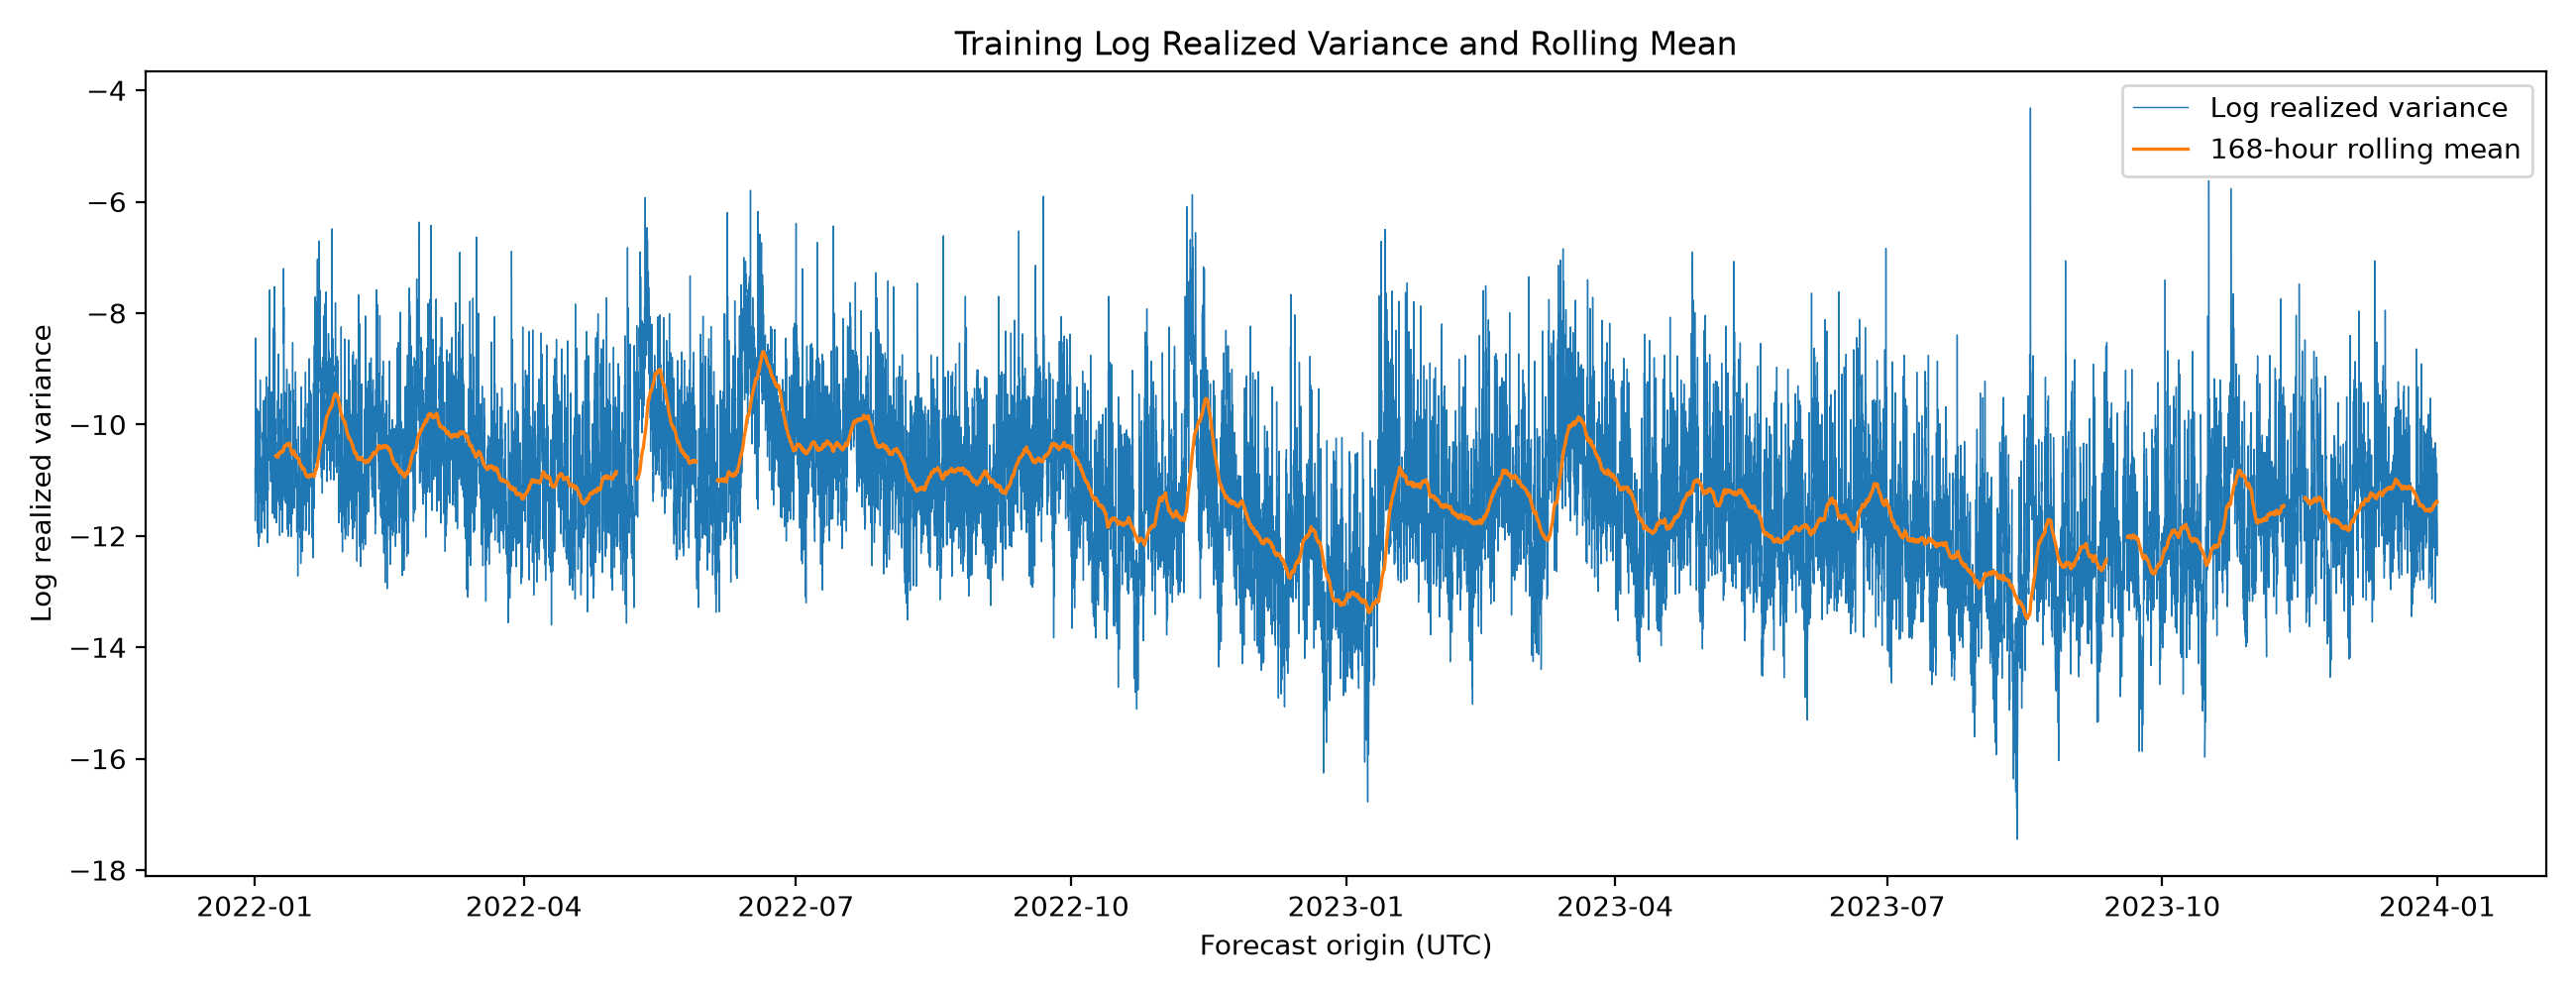
\includegraphics[
    width=0.95\textwidth
]
{../outputs/figures/training_log_rv_and_rolling_mean.png}
\caption{
Training-period log realized variance and its 168-hour
rolling mean
}
\label{fig:training-log-rv}
\end{figure}
}
{}

Log realized variance repeatedly returns toward its prevailing
level after large increases, indicating mean-reverting
behavior. The rolling mean nevertheless changes over the
training period, suggesting that the unconditional level is
not constant throughout the sample.

Table~\ref{tab:stationarity-tests} reports the formal test
results.

\begin{table}[H]
\centering
\caption{Training-period stationarity tests}
\label{tab:stationarity-tests}
\begin{tabular}{lrrrrl}
\toprule
Test
& Statistic
& \(p\)-value
& Lags
& Observations
& Decision at 5\% \\
\midrule
ADF
& -8.0186
& \(<0.001\)
& 40
& 11,277
& Reject unit root \\

KPSS
& 5.9013
& 0.010
& 57
& 11,318
& Reject level stationarity \\
\bottomrule
\end{tabular}
\end{table}

The augmented Dickey--Fuller test strongly rejects the
unit-root null \citep{saiddickey1984}, providing evidence of
mean reversion. The KPSS test also rejects global level
stationarity \citep{kpss1992}. Taken together, the results
indicate a persistent and mean-reverting series whose level or
dependence structure changes over longer periods.

These findings support the use of a fixed autoregression as a
forecasting benchmark while also motivating a specification
that allows gradual parameter variation.

\IfFileExists
{../outputs/figures/training_log_rv_acf.png}
{
\begin{figure}[H]
\centering
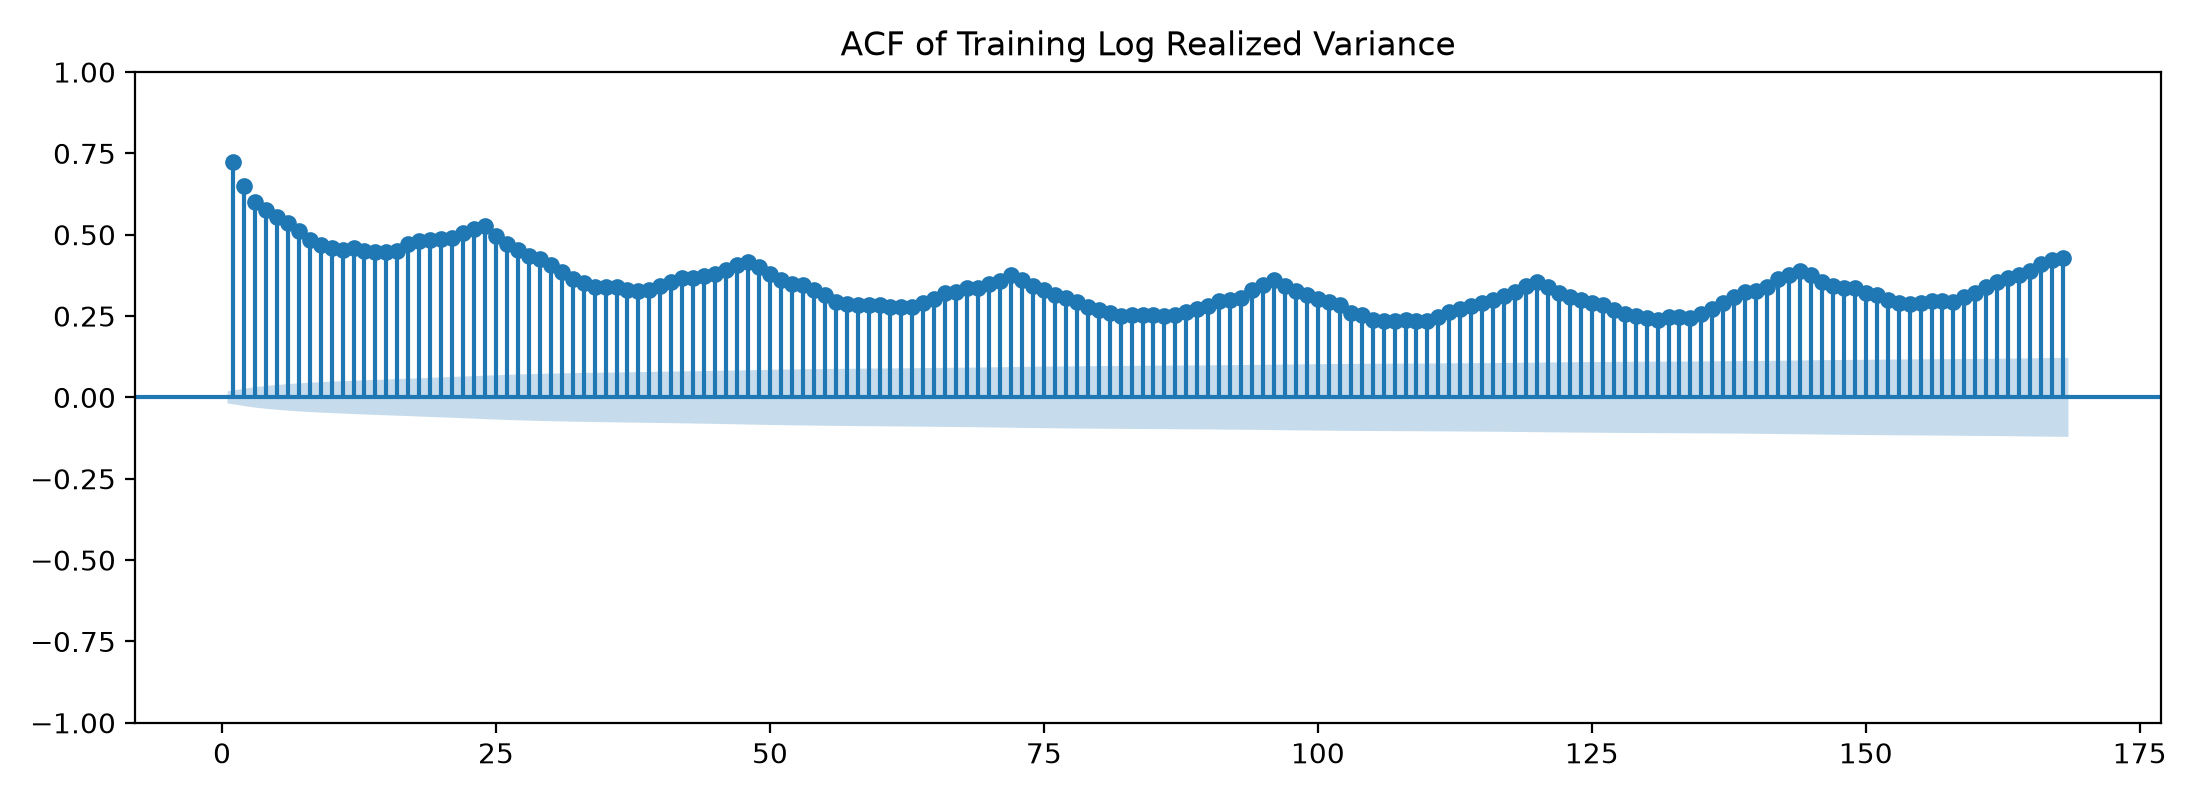
\includegraphics[
    width=0.92\textwidth
]
{../outputs/figures/training_log_rv_acf.png}
\caption{
Autocorrelation function of training-period log realized
variance
}
\label{fig:training-acf}
\end{figure}
}
{}

Figure~\ref{fig:training-acf} shows substantial
autocorrelation beyond the first few hours. The persistence
benchmark therefore captures only part of the temporal
dependence in hourly volatility.

\subsection{Autoregressive Order Selection}

AR orders from 1 through 24 are estimated on the training
sample and ranked by validation QLIKE. Table
\ref{tab:ar-order-selection} reports the five leading
specifications.

\begin{table}[H]
\centering
\caption{Leading AR specifications ranked by validation QLIKE}
\label{tab:ar-order-selection}
\begin{tabular}{rrrrrr}
\toprule
Order
& Training AIC
& Training BIC
& Validation MAE
& Validation RMSE
& Validation QLIKE \\
\midrule
24 & 43,353.53 & 43,546.57 & 0.6219 & 0.8023 & 0.5105 \\
23 & 43,392.98 & 43,578.29 & 0.6232 & 0.8037 & 0.5122 \\
22 & 43,455.91 & 43,633.50 & 0.6253 & 0.8061 & 0.5143 \\
21 & 43,528.03 & 43,697.90 & 0.6267 & 0.8080 & 0.5161 \\
20 & 43,557.89 & 43,720.04 & 0.6277 & 0.8090 & 0.5196 \\
\bottomrule
\end{tabular}
\end{table}

AR(24) achieves the lowest validation QLIKE, RMSE, and MAE
and is selected as the autoregressive benchmark. Its position
at the upper boundary of the candidate set suggests that
information from the preceding 24 hours remains useful. The
incremental gains decline as the order increases, indicating
that predictive dependence is distributed across several lags
rather than concentrated in a single hour.

The validation losses for AR(24) are \(0.6219\) for MAE,
\(0.8023\) for RMSE, and \(0.5105\) for QLIKE. Relative to
persistence, these values represent reductions of
approximately \(13.14\%\), \(12.59\%\), and \(21.22\%\),
respectively. Estimated lag dynamics therefore provide
substantial predictive value beyond the current volatility
level.

\subsubsection{AR Stability and Residual Diagnostics}

All characteristic roots of AR(24) lie outside the unit
circle. The minimum root modulus is \(1.0084\), indicating a
stable but highly persistent specification.

The first-order residual autocorrelation is \(0.0036\).
Ljung--Box portmanteau tests nevertheless reject residual white
noise at lags 29, 48, and 168, with \(p\)-values below
\(0.001\) \citep{ljungbox1978}.

AR(24) captures most immediate dependence but leaves weaker
correlation at longer horizons. It therefore provides a strong
forecasting benchmark while leaving scope for the
multi-horizon HAR-X specification.

\subsection{Fixed HAR-X Estimation Results}

Fixed HAR-X combines multi-horizon volatility components with
downside semivariance, trading activity, and aggressive-buying
information. Table~\ref{tab:fixed-harx-coefficients} reports
standardized coefficients with Newey--West HAC standard errors
\citep{neweywest1987}.

\begin{table}[H]
\centering
\caption{
Fixed HAR-X standardized coefficients with HAC(24) inference
}
\label{tab:fixed-harx-coefficients}
\scriptsize
\begin{tabular}{p{5.7cm}rrrr}
\toprule
Predictor
& Coefficient
& HAC standard error
& \(t\)-statistic
& \(p\)-value \\
\midrule
Current-hour volatility
& 0.2616
& 0.0239
& 10.94
& \(<0.001\) \\

Six-hour volatility
& 0.2632
& 0.0167
& 15.73
& \(<0.001\) \\

Twenty-four-hour volatility
& 0.2574
& 0.0183
& 14.09
& \(<0.001\) \\

One-hundred-sixty-eight-hour volatility
& 0.1163
& 0.0140
& 8.31
& \(<0.001\) \\

Transformed downside semivariance
& -0.0062
& 0.0192
& -0.32
& 0.745 \\

Log number of trades
& 0.3379
& 0.0153
& 22.13
& \(<0.001\) \\

Aggressive-buying proxy
& -0.0006
& 0.0088
& -0.07
& 0.948 \\
\bottomrule
\end{tabular}
\end{table}

All four HAR components have positive and statistically
significant coefficients, consistent with the
heterogeneous-horizon representation of realized volatility
\citep{corsi2009}. Current, intraday, daily, and weekly
volatility each contribute information after conditioning on
the remaining predictors.

Trading activity has a coefficient of \(0.3379\) and is highly
significant. Because the predictors are standardized, a
one-standard-deviation increase in log trade count is
associated with an increase of approximately \(0.338\) in
next-hour log realized variance, conditional on the other
variables.

This result is consistent with the information-arrival
interpretation of trading activity \citep{clark1973} and the
documented relationship between transaction counts and
volatility \citep{jones1994}. Among the three additional
market-activity variables, trade count provides the strongest
incremental predictive evidence.

The coefficients on downside semivariance and aggressive
buying are small and statistically insignificant. Their
average conditional associations with next-hour volatility are
therefore weak over the estimation period.

All coefficient estimates are interpreted as predictive
associations.

\subsection{Fixed HAR-X Validation Performance}

Table~\ref{tab:validation-model-comparison} compares the four
models on the validation sample.

\begin{table}[H]
\centering
\caption{Validation-period forecast performance}
\label{tab:validation-model-comparison}
\begin{tabular}{lrrrr}
\toprule
Model
& MAE
& RMSE
& QLIKE
& QLIKE improvement vs.\ Naive \\
\midrule
Naive
& 0.7160
& 0.9179
& 0.6480
& 0.00\% \\

AR(24)
& 0.6219
& 0.8023
& 0.5105
& 21.22\% \\

Fixed HAR-X
& 0.6106
& 0.7913
& 0.5083
& 21.56\% \\

TVP-HAR-X
& 0.6079
& 0.7857
& 0.4864
& 24.93\% \\
\bottomrule
\end{tabular}
\end{table}

Fixed HAR-X improves on AR(24) under all three metrics. The
QLIKE reduction is \(0.42\%\), showing that AR(24) already
captures much of the predictive content in recent volatility.

Fixed HAR-X achieves this performance with seven structured
predictors and incorporates information extending to the
preceding week. The specification therefore provides a
parsimonious and interpretable alternative to a larger set of
individual hourly lags.

Its residual first-order autocorrelation is close to zero, and
the Durbin--Watson statistic is \(2.009\). Ljung--Box tests
remain significant at lags 24, 48, and 168, indicating
residual dependence at longer horizons.

\subsection{TVP-HAR-X Parameter Estimates}

The TVP-HAR-X variance parameters are estimated on the
training sample by maximizing the Kalman-filter
prediction-error likelihood \citep{durbin2012}. Three sets of
starting values converge to nearly identical solutions,
indicating numerical stability.

\begin{table}[H]
\centering
\caption{Training-period TVP-HAR-X variance parameters}
\label{tab:tvp-variance-parameters}
\begin{tabular}{lrr}
\toprule
Parameter
& Variance
& Standard deviation \\
\midrule
Observation disturbance
& \(7.4918\times10^{-1}\)
& \(8.6555\times10^{-1}\) \\

Intercept-state innovation
& \(2.5406\times10^{-5}\)
& \(5.0404\times10^{-3}\) \\

Common slope-state innovation
& \(1.6681\times10^{-6}\)
& \(1.2915\times10^{-3}\) \\
\bottomrule
\end{tabular}
\end{table}

Both state innovation variances are small relative to the
observation variance, producing gradual coefficient movement.
The intercept innovation standard deviation exceeds the common
slope innovation standard deviation, indicating faster
variation in the overall volatility level than in the marginal
predictor effects.

The estimated state variances are positive, so the fitted model
does not collapse numerically to a fixed-coefficient
specification.

\subsection{Time-Varying Coefficient Behavior}

Table~\ref{tab:tvp-state-summary} summarizes the predicted
state estimates during validation.

\begin{table}[H]
\centering
\caption{Validation-period time-varying coefficient summary}
\label{tab:tvp-state-summary}
\scriptsize
\begin{tabular}{p{5.3cm}rrrr}
\toprule
State
& Mean
& Standard deviation
& Minimum
& Maximum \\
\midrule
Intercept
& -11.2035
& 0.0936
& -11.4340
& -10.9837 \\

Current-hour volatility
& 0.1102
& 0.0312
& 0.0502
& 0.1918 \\

Six-hour volatility
& 0.2447
& 0.0194
& 0.1988
& 0.2976 \\

Twenty-four-hour volatility
& 0.1721
& 0.0271
& 0.1203
& 0.2514 \\

One-hundred-sixty-eight-hour volatility
& 0.0076
& 0.0316
& -0.0781
& 0.0576 \\

Transformed downside semivariance
& -0.0175
& 0.0508
& -0.1261
& 0.0787 \\

Log number of trades
& 0.5336
& 0.0528
& 0.4407
& 0.6513 \\

Aggressive-buying proxy
& -0.0324
& 0.0232
& -0.0864
& 0.0373 \\
\bottomrule
\end{tabular}
\end{table}

Trading activity has the largest average positive coefficient
and remains positive throughout validation, ranging from
approximately \(0.441\) to \(0.651\). It is therefore a
consistently informative predictor within this period.

The six-hour and twenty-four-hour coefficients also remain
positive and vary within relatively narrow ranges. Short- and
medium-horizon volatility persistence is consequently stable
during validation.

The weekly coefficient fluctuates around zero, while the
downside-semivariance and aggressive-buying coefficients
change sign. Their predictive contributions vary more
substantially across the sample.

The state paths describe changes in conditional forecasting
relationships and are not assigned a causal interpretation.

\subsection{TVP-HAR-X Validation Performance}

TVP-HAR-X records validation MAE of \(0.6079\), RMSE of
\(0.7857\), and QLIKE of \(0.4864\). QLIKE is \(4.30\%\)
lower than for Fixed HAR-X and \(24.93\%\) lower than for the
persistence benchmark.

The standardized innovations have a mean of approximately
\(-0.0095\), a standard deviation of \(1.024\), and
first-order autocorrelation of \(0.0007\). These values are
close to the corresponding theoretical benchmarks of zero,
one, and zero.

Longer-horizon Ljung--Box tests remain significant. Given the
large diagnostic sample, these rejections reflect small
autocorrelations accumulated across several lags. The
state-space model improves validation forecasts while leaving
some temporal dependence unexplained.

\subsection{Final Out-of-Sample Test Results}

After model selection, AR(24), Fixed HAR-X, and TVP-HAR-X
are re-estimated using the combined training and validation
sample. The locked specifications are then evaluated on
\(8{,}422\) common test observations from 2025.

Table~\ref{tab:final-test-results} reports the final
out-of-sample performance.

\begin{table}[H]
\centering
\caption{Final 2025 test-set forecast performance}
\label{tab:final-test-results}
\begin{tabular}{lrrrrrr}
\toprule
Model
& MAE
& MAE rank
& RMSE
& RMSE rank
& QLIKE
& QLIKE rank \\
\midrule
Naive
& 0.7021
& 4
& 0.9101
& 4
& 0.7007
& 4 \\

AR(24)
& 0.6133
& 3
& 0.7997
& 3
& 0.5054
& 3 \\

Fixed HAR-X
& 0.5980
& 2
& 0.7807
& 2
& \textbf{0.4764}
& \textbf{1} \\

TVP-HAR-X
& \textbf{0.5901}
& \textbf{1}
& \textbf{0.7734}
& \textbf{1}
& 0.4800
& 2 \\
\bottomrule
\end{tabular}
\end{table}

All three estimated models improve substantially on
persistence. Relative to Naive, test QLIKE falls by
\(27.87\%\) for AR(24), \(32.02\%\) for Fixed HAR-X, and
\(31.50\%\) for TVP-HAR-X.

Fixed HAR-X reduces QLIKE by \(5.75\%\) relative to AR(24).
The structured multi-horizon and market-activity predictors
therefore provide additional forecasting information beyond
the 24 hourly lags.

The ranking of the two HAR-X models varies across loss
functions. TVP-HAR-X records the lowest MAE and RMSE, while
Fixed HAR-X records the lowest QLIKE. Relative to Fixed HAR-X,
TVP-HAR-X reduces absolute error by \(1.33\%\) and squared
error by \(1.87\%\). Its QLIKE is \(0.76\%\) higher.

\IfFileExists
{../outputs/figures/final_test_mae_comparison.png}
{
\begin{figure}[H]
\centering
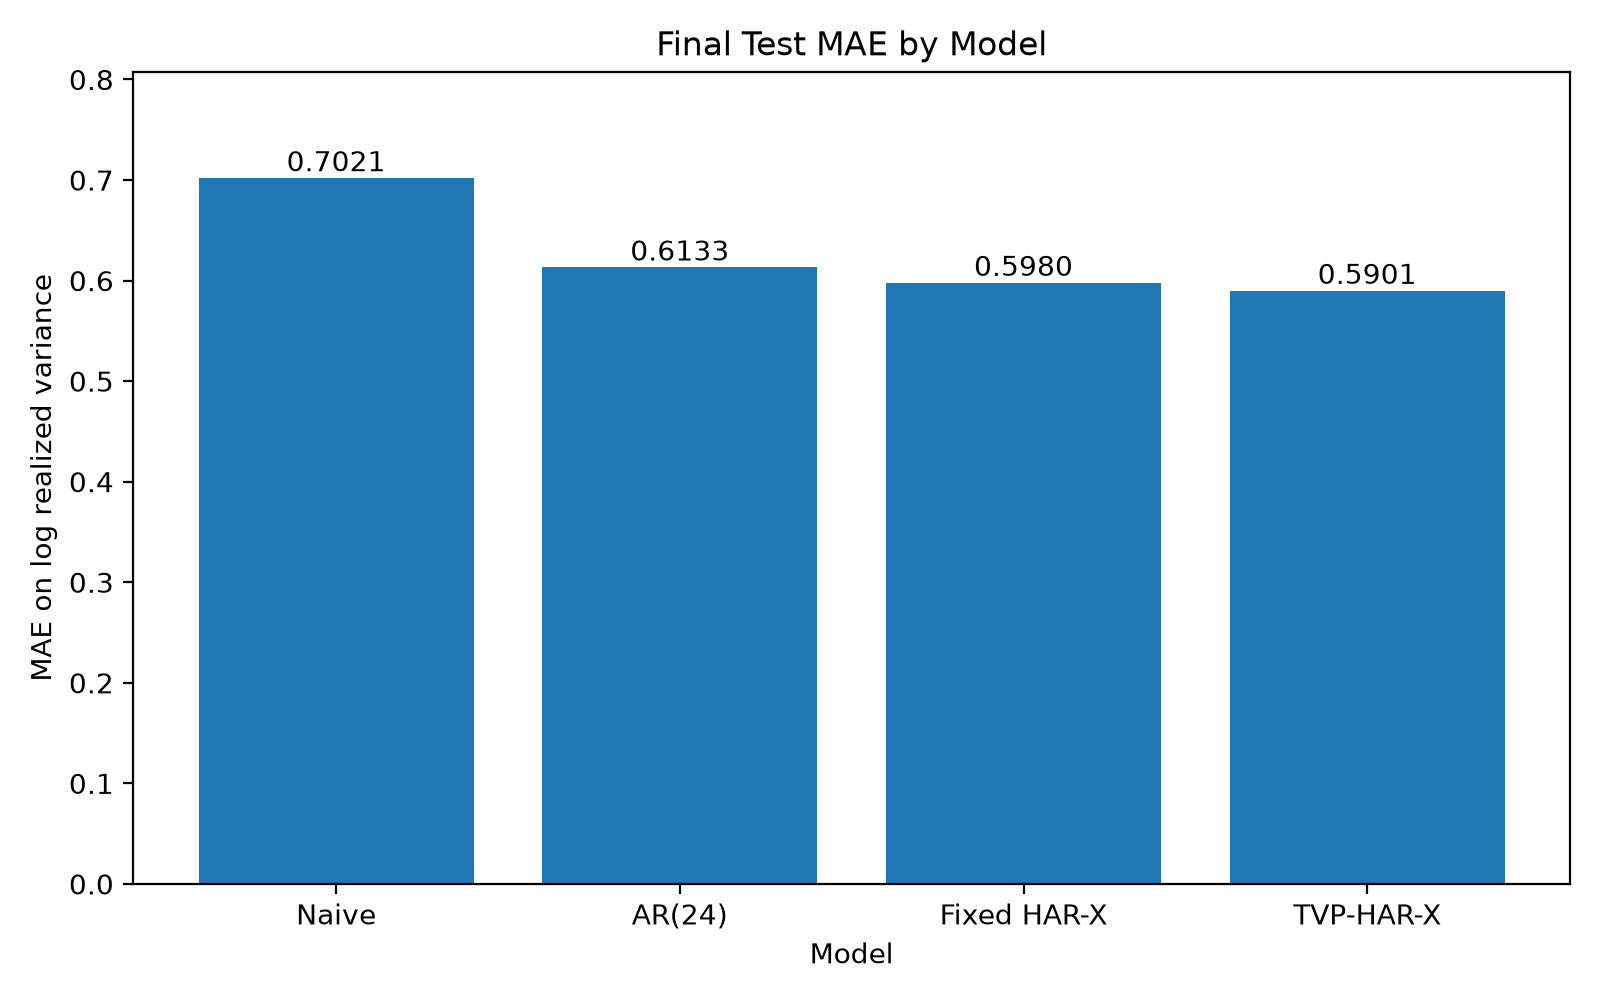
\includegraphics[
    width=0.80\textwidth
]
{../outputs/figures/final_test_mae_comparison.png}
\caption{Final test MAE across forecasting models}
\label{fig:final-mae}
\end{figure}
}
{}

\IfFileExists
{../outputs/figures/final_test_rmse_comparison.png}
{
\begin{figure}[H]
\centering
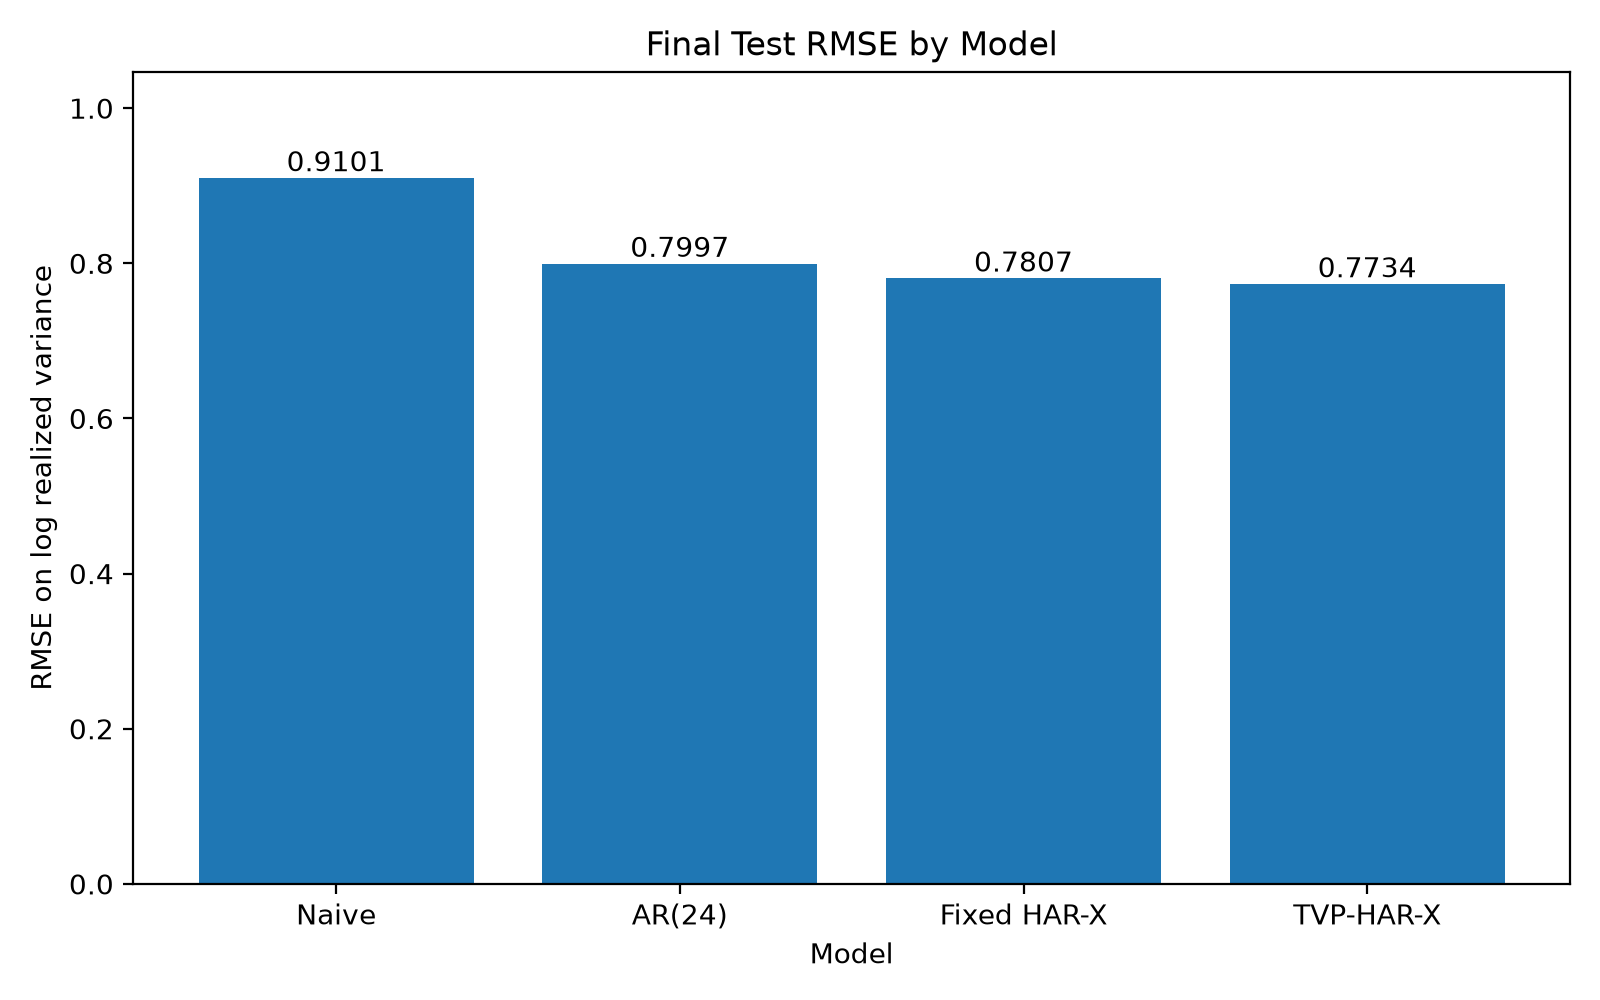
\includegraphics[
    width=0.80\textwidth
]
{../outputs/figures/final_test_rmse_comparison.png}
\caption{Final test RMSE across forecasting models}
\label{fig:final-rmse}
\end{figure}
}
{}

\IfFileExists
{../outputs/figures/final_test_qlike_comparison.png}
{
\begin{figure}[H]
\centering
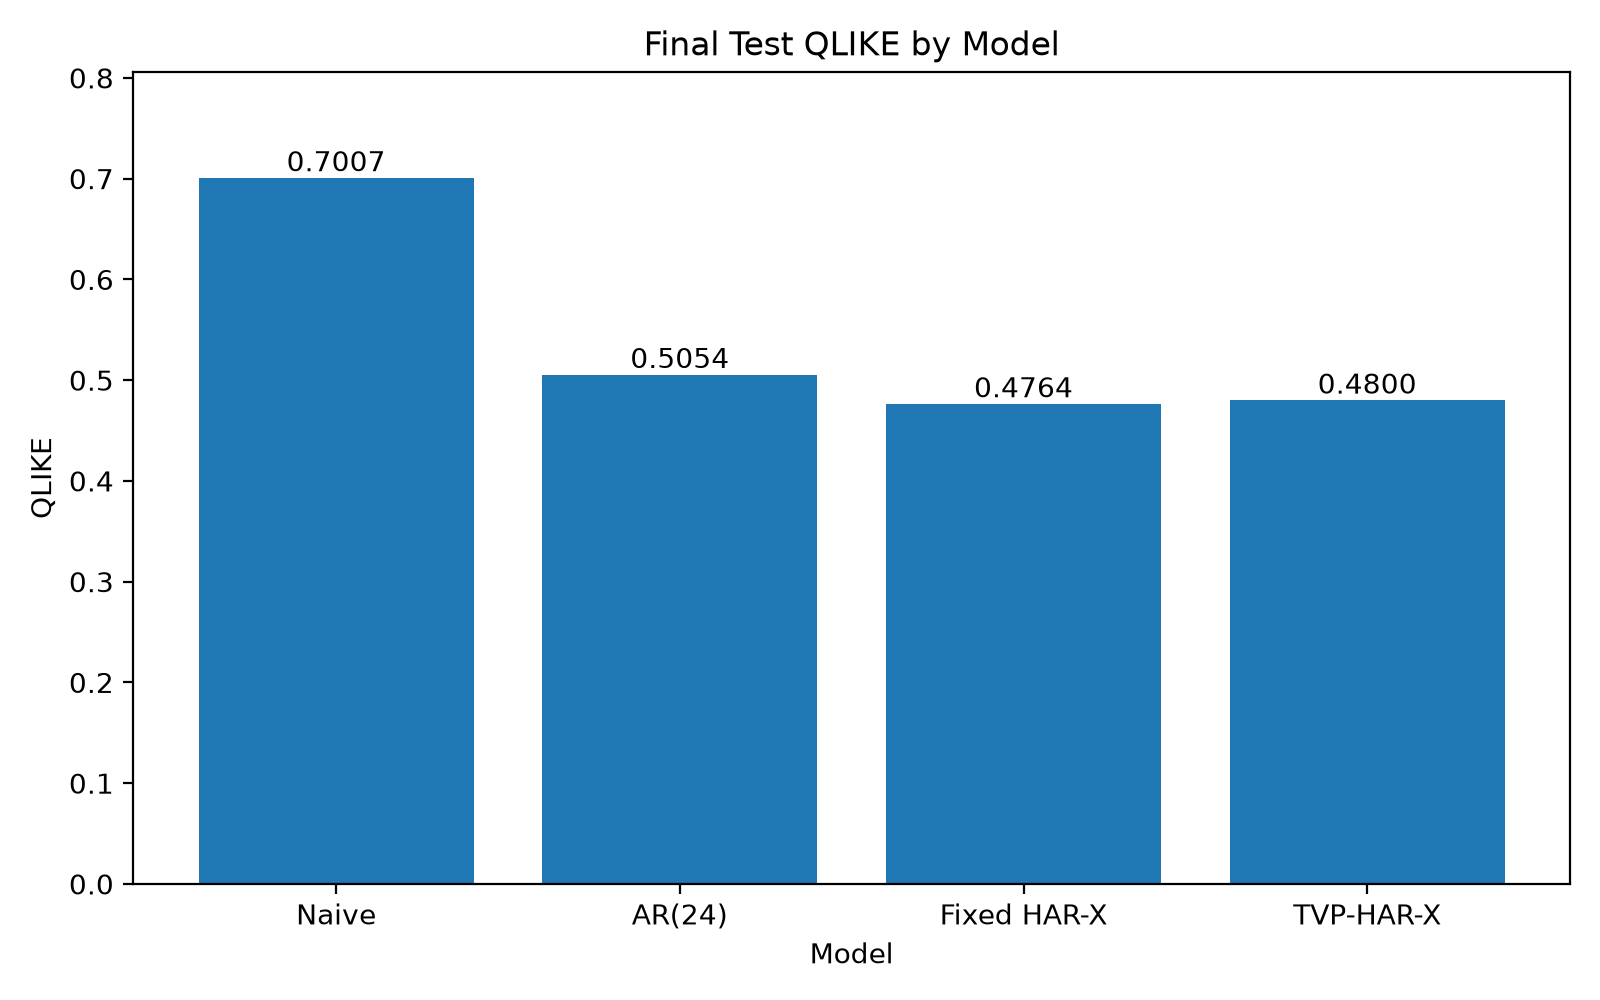
\includegraphics[
    width=0.80\textwidth
]
{../outputs/figures/final_test_qlike_comparison.png}
\caption{Final test QLIKE across forecasting models}
\label{fig:final-qlike}
\end{figure}
}
{}

Figures~\ref{fig:final-mae}--\ref{fig:final-qlike} show that
the difference between the two HAR-X specifications is small
relative to their gains over Naive and AR(24). They also
illustrate the change in ranking between log-scale errors and
variance-scale loss.

\subsection{Predictive-Loss Significance Tests}

Table~\ref{tab:tvp-fixed-loss-tests} reports
Diebold--Mariano-type loss-differential tests
\citep{dieboldmariano1995} using Newey--West HAC standard
errors \citep{neweywest1987}. The loss differential is defined
so that positive values favor TVP-HAR-X.

\begin{table}[H]
\centering
\caption{
HAC loss-differential tests:
TVP-HAR-X versus Fixed HAR-X
}
\label{tab:tvp-fixed-loss-tests}
\begin{tabular}{lrrrrl}
\toprule
Loss
& Fixed HAR-X
& TVP-HAR-X
& Improvement
& Test statistic
& One-sided \(p\)-value \\
\midrule
Absolute error
& 0.5980
& 0.5901
& 1.33\%
& 6.2596
& \(<0.001\) \\

Squared error
& 0.6096
& 0.5981
& 1.87\%
& 6.0210
& \(<0.001\) \\

QLIKE
& 0.4764
& 0.4800
& -0.76\%
& -1.2118
& 0.887 \\
\bottomrule
\end{tabular}
\end{table}

TVP-HAR-X significantly reduces absolute and squared loss
relative to Fixed HAR-X. The corresponding one-sided
\(p\)-values are below \(0.001\).

The QLIKE loss differential has a mean of \(-0.00362\) and a
one-sided \(p\)-value of \(0.887\). The test therefore provides
no evidence that TVP-HAR-X improves on Fixed HAR-X under the
pre-specified primary loss. The negative point estimate is
consistent with the lower QLIKE reported for Fixed HAR-X.

TVP-HAR-X also improves significantly on Naive and AR(24)
under all three losses. Its test QLIKE is approximately
\(5.03\%\) lower than that of AR(24), with a one-sided
\(p\)-value below \(0.001\).

\subsection{Validation--Test Comparison}

The relative performance of Fixed HAR-X and TVP-HAR-X changes
between the validation and test periods. TVP-HAR-X reduces
validation QLIKE by \(4.30\%\) relative to Fixed HAR-X, whereas
its test QLIKE is \(0.76\%\) higher.

This change in ranking shows that the validation advantage of
the time-varying specification does not persist uniformly
through the test period.

\IfFileExists
{../outputs/figures/final_test_monthly_qlike.png}
{
\begin{figure}[H]
\centering
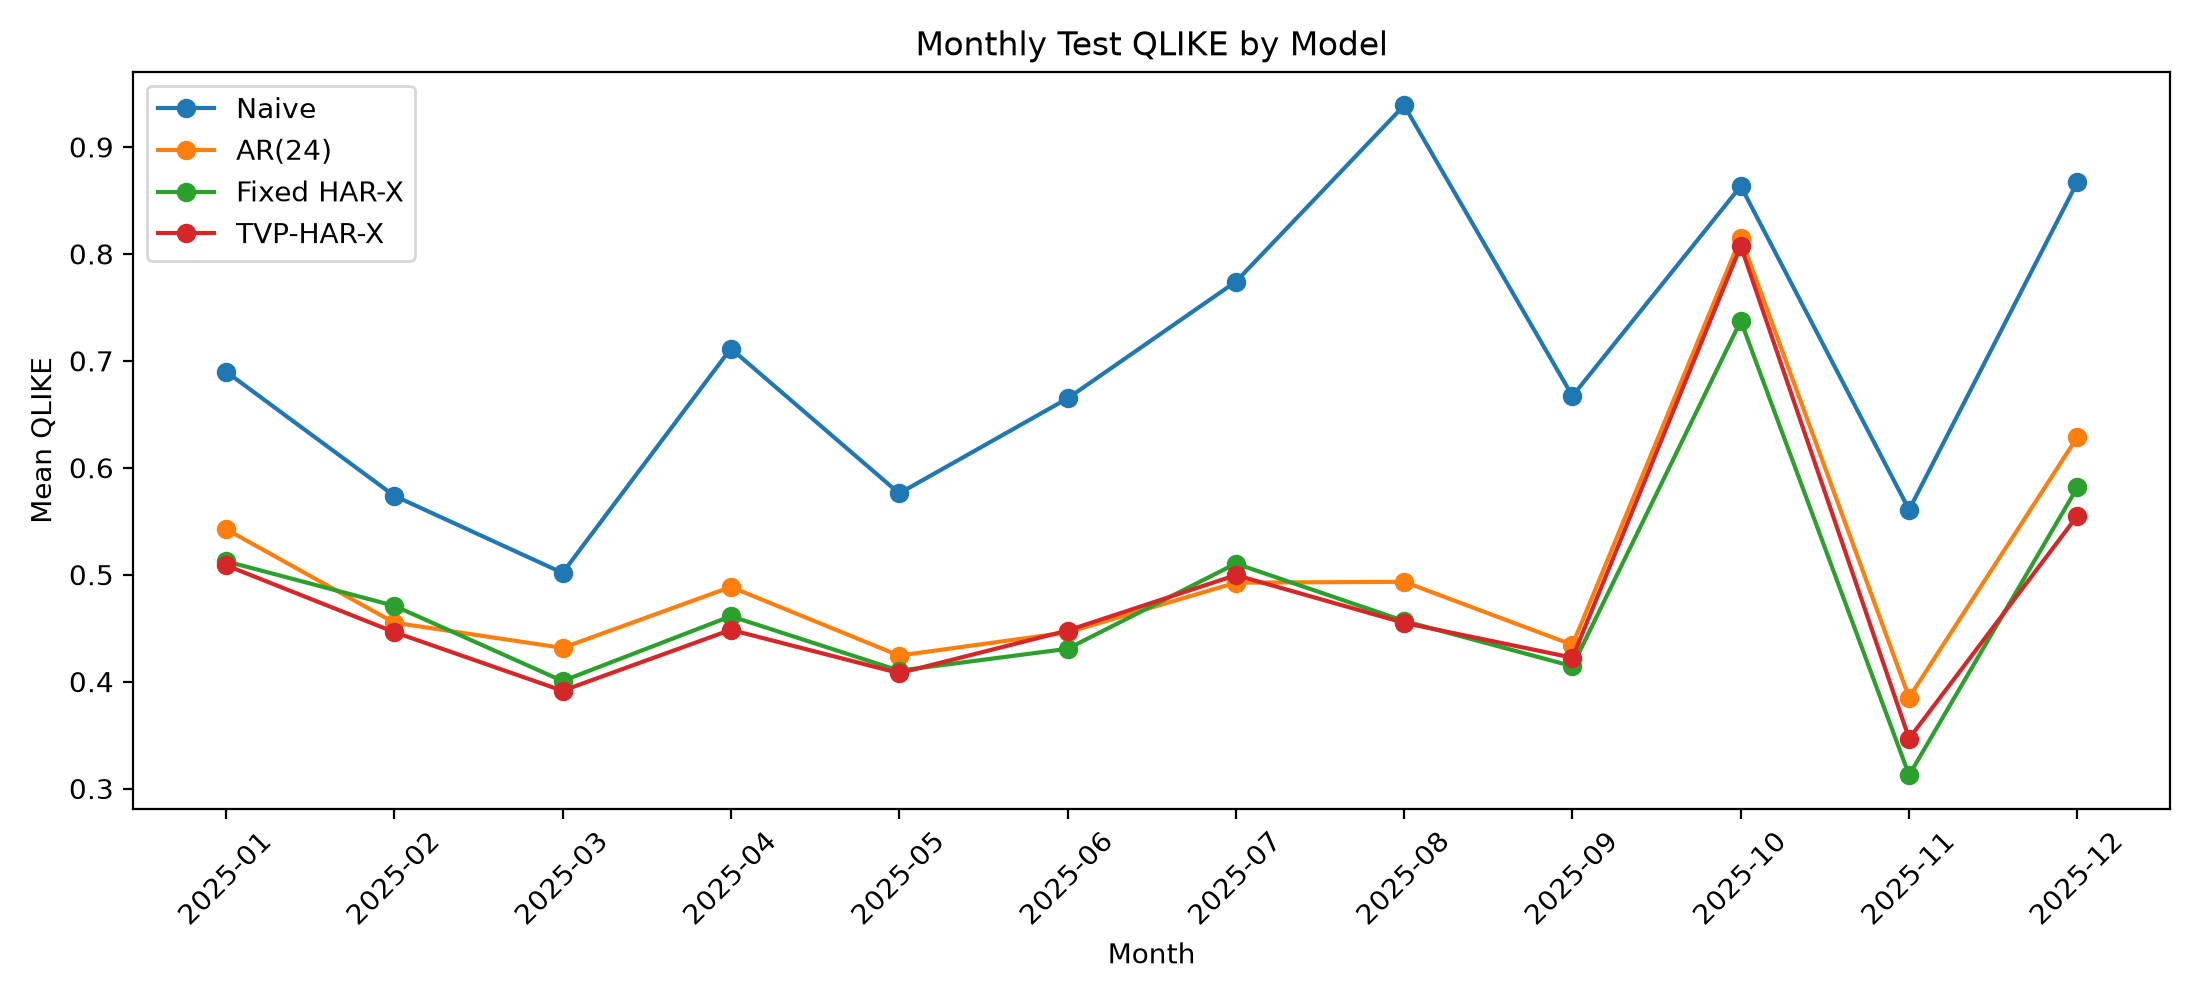
\includegraphics[
    width=0.94\textwidth
]
{../outputs/figures/final_test_monthly_qlike.png}
\caption{Monthly test-period QLIKE by model}
\label{fig:monthly-qlike}
\end{figure}
}
{}

Figure~\ref{fig:monthly-qlike} reports monthly QLIKE during
2025. The ranking of Fixed HAR-X and TVP-HAR-X varies across
months, so the annual averages combine periods with different
relative performance.

\IfFileExists
{../outputs/figures/final_test_cumulative_qlike_difference_fixed_vs_tvp.png}
{
\begin{figure}[H]
\centering
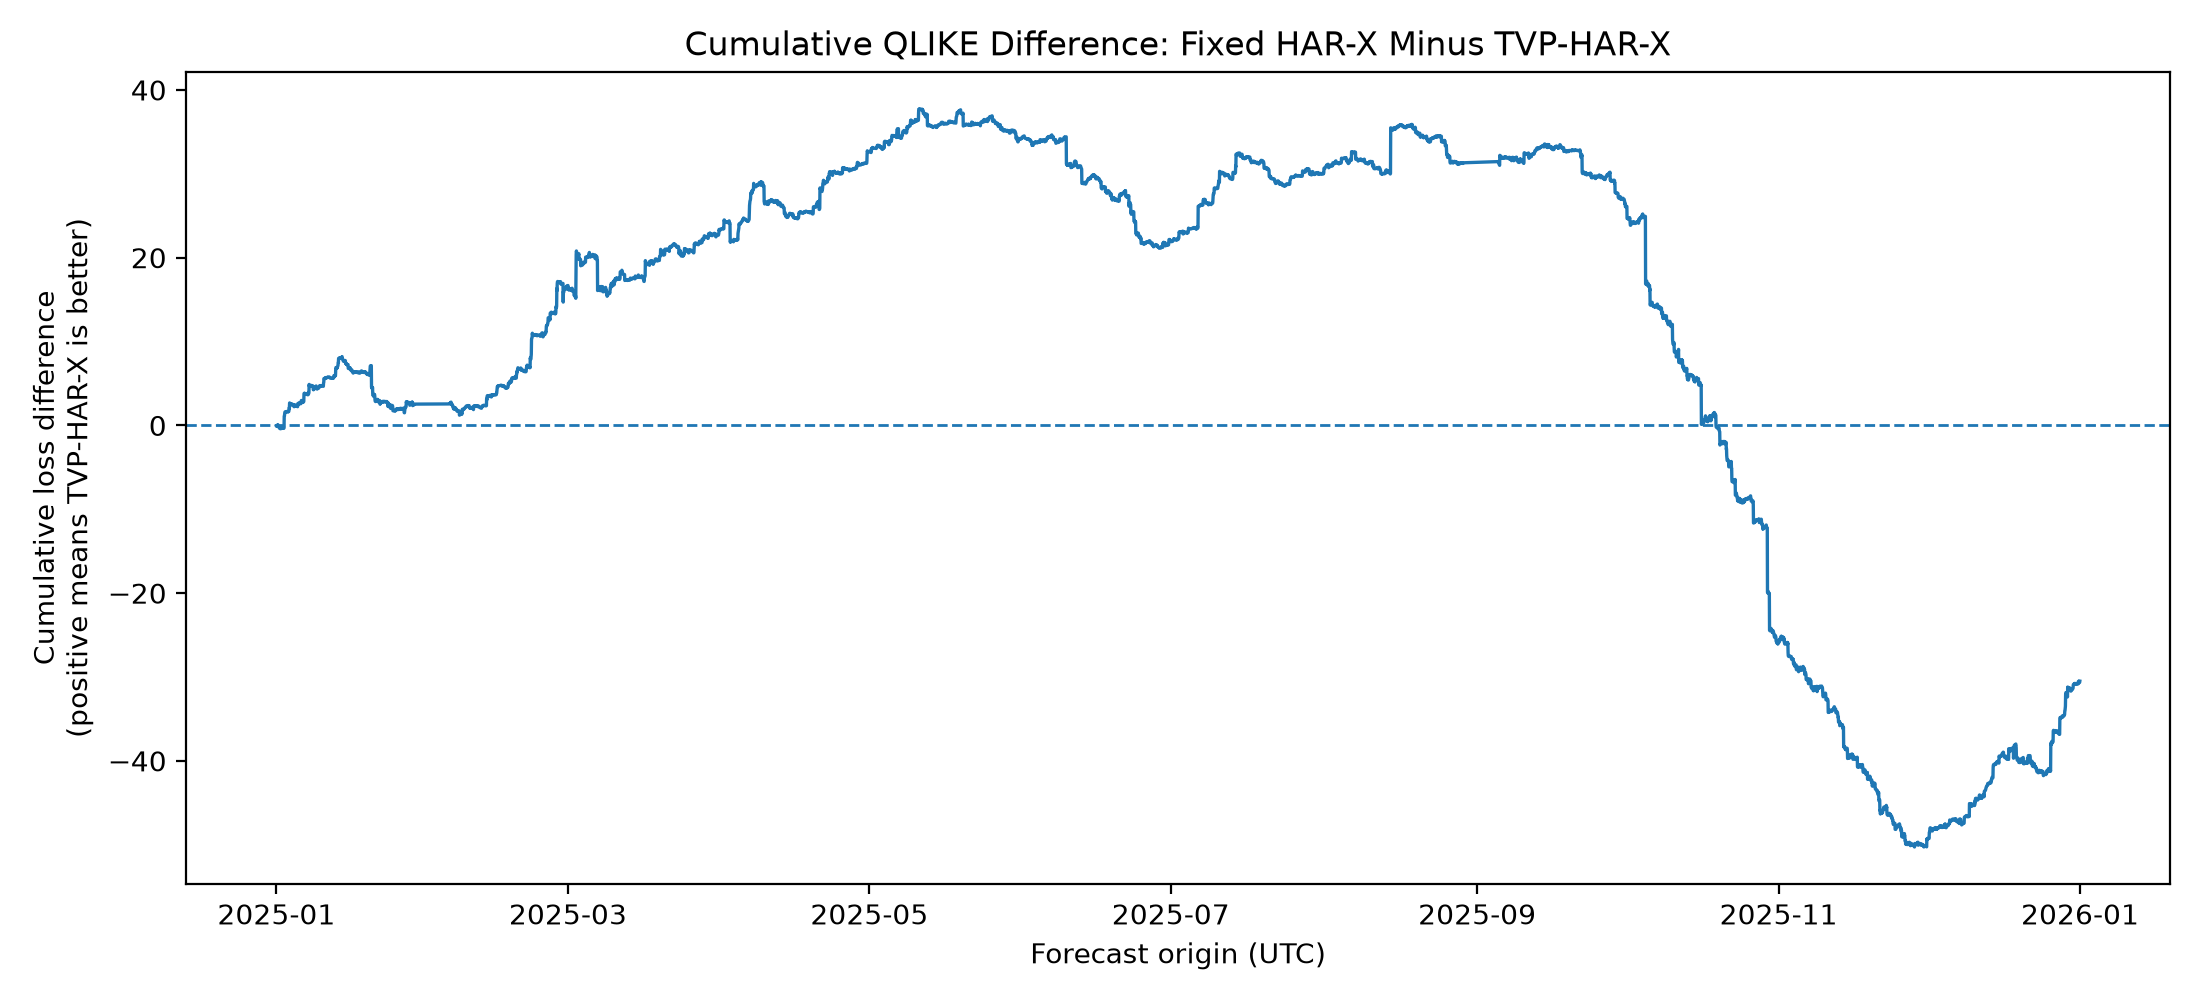
\includegraphics[
    width=0.94\textwidth
]
{../outputs/figures/final_test_cumulative_qlike_difference_fixed_vs_tvp.png}
\caption{
Cumulative QLIKE difference between Fixed HAR-X and TVP-HAR-X
}
\label{fig:cumulative-qlike-difference}
\end{figure}
}
{}

Figure~\ref{fig:cumulative-qlike-difference} displays the
cumulative difference between Fixed HAR-X and TVP-HAR-X
QLIKE. An upward segment indicates lower loss for TVP-HAR-X,
while a downward segment indicates lower loss for Fixed HAR-X.
The path confirms that neither specification maintains a
uniform advantage throughout the test year.

\subsection{Summary of Empirical Findings}

The empirical results yield five main findings.

\begin{enumerate}[label=(\arabic*)]

    \item
    Hourly log realized variance is persistent and mean
    reverting, although global level stationarity is rejected.

    \item
    AR(24) improves substantially on persistence, indicating
    that predictive dependence extends across several recent
    hours.

    \item
    Fixed HAR-X improves on AR(24), particularly under test
    QLIKE, supporting the use of multi-horizon volatility and
    market-activity predictors.

    \item
    Trading activity provides the strongest incremental
    predictor among the additional HAR-X variables.

    \item
    TVP-HAR-X achieves the lowest MAE and RMSE, while Fixed
    HAR-X achieves the lowest QLIKE. The gains from parameter
    variation therefore depend on the evaluation criterion.

\end{enumerate}

The strongest and most stable improvement arises from moving
from persistence and AR(24) to the HAR-X information set.
Time-varying coefficients provide additional gains in
log-scale forecast accuracy, while the fixed specification
performs best under the primary variance-scale loss.

\section{Discussion}
\label{sec:discussion}
\subsection{Interpretation of the Main Result}

The final test results produce different rankings across the
three loss functions. TVP-HAR-X achieves the lowest MAE and
RMSE on the log realized-variance scale, whereas Fixed HAR-X
achieves the lowest QLIKE on the original variance scale.

MAE and RMSE evaluate errors in
\(y_t=\log(RV_t)\). MAE summarizes the typical absolute
deviation, while RMSE assigns greater weight to large
log-scale errors.

QLIKE evaluates the implied variance forecast
\(\widehat{RV}_t=\exp(\widehat{y}_t)\). Its loss depends on the
ratio \(RV_t/\widehat{RV}_t\), making it particularly sensitive
to substantial underprediction during high-volatility periods
\citep{patton2011}. A model may therefore reduce average
log-scale errors while recording a higher QLIKE because of a
small number of unfavorable variance forecasts.

The test results suggest that coefficient adaptation improves
the typical accuracy of log-volatility forecasts. Fixed HAR-X,
however, provides slightly better performance under the
variance-scale loss. The empirical value of parameter
variation consequently depends on the forecasting objective.

\subsection{Validation and Test Performance}

TVP-HAR-X reduces validation QLIKE by approximately \(4.30\%\)
relative to Fixed HAR-X, but its test QLIKE is \(0.76\%\)
higher. This change in ranking illustrates the importance of
retaining a separate final test period.

Fixed HAR-X estimates a single coefficient vector from the
development sample and produces relatively stable forecasts.
TVP-HAR-X introduces gradual coefficient movement, reducing
bias when predictive relationships change while adding
state-estimation uncertainty.

The relative performance of the two specifications can be
understood as a trade-off between adaptation and estimation
uncertainty. During validation, parameter variation improves
all three losses. During the test period, it continues to
reduce MAE and RMSE, but the gain is insufficient to lower
QLIKE.

The difference across years also indicates that forecast-model
rankings are sensitive to market conditions. Chronological
validation is therefore more informative than a random split
for this application.

\subsection{Incremental Value of the HAR-X Information Set}

The most substantial model improvement occurs between AR(24)
and Fixed HAR-X. On the final test sample, Fixed HAR-X reduces
QLIKE by approximately \(5.75\%\) relative to AR(24).

AR(24) is a demanding benchmark because it estimates a
separate coefficient for each of the previous 24 hourly
volatility observations. The HAR-X improvement therefore
provides evidence that the structured predictor set contains
information beyond an unrestricted one-day lag specification.

The HAR variables extend the information set to the preceding
week without requiring 168 individual lag coefficients. This
multi-horizon representation follows the HAR framework of
\citet{corsi2009} and provides a parsimonious description of
persistent volatility.

HAR-X also incorporates current market activity. Among the
additional variables, log trade count displays the strongest
and most stable association with next-hour volatility. The
forecasting information set thus combines recent volatility,
longer-horizon volatility conditions, and current trading
activity.

\subsection{Interpretation of Trading Activity}

Trading activity is the most informative additional predictor
in both HAR-X specifications. In the fixed model, its
standardized coefficient is \(0.3379\), with a HAC
\(p\)-value below \(0.001\). During validation, its
time-varying coefficient remains positive and ranges from
approximately \(0.441\) to \(0.651\).

These estimates indicate that unusually active trading hours
tend to be followed by higher next-hour log realized variance,
conditional on volatility measured at the four HAR horizons.

The result is consistent with the interpretation of trade
count as a proxy for information arrival and market attention.
It is related to the mixture-of-distributions framework of
\citet{clark1973} and the transaction-count evidence reported
by \citet{jones1994}. Increased activity may reflect periods
in which market participants are processing new information
and adjusting positions more intensively.

The estimated coefficient represents a conditional predictive
association. Trading activity and volatility may respond
jointly to latent information or broader changes in market
conditions, so the model does not identify a causal effect.

\subsection{Downside Semivariance}

Downside semivariance is statistically insignificant in the
fixed HAR-X model, and its time-varying coefficient changes
sign during validation.

Realized semivariance separates the contributions of negative
and positive intraday returns to total variation
\citep{barndorffnielsen2010}. In the present specification,
total realized variance and the current-hour HAR component
already contain the squared magnitudes of both positive and
negative returns. Downside semivariance must therefore provide
information beyond the overall volatility level to obtain a
distinct effect.

The estimates suggest that this additional contribution is
small on average at the one-hour forecast horizon. The
logarithmic transformation may also reduce the influence of a
limited number of extreme downside observations. The
time-varying estimates do not reveal a persistent positive or
negative relationship.

\subsection{Aggressive-Buying Proxy}

The aggressive-buying proxy has a coefficient close to zero in
the fixed model and changes sign in the TVP specification.

The signed measure records the balance between taker-initiated
buying and selling. Large imbalances in either direction may
coincide with elevated volatility, which can weaken the average
linear effect of a signed variable.

An absolute or nonlinear imbalance measure could capture this
possibility more directly. Such alternatives were not included
in the pre-specified model and would require evaluation on a
new holdout sample.

The weak result may also reflect the information available in
candlestick data. Aggregated taker-buy volume does not capture
order-book depth, bid--ask spreads, cancellations, or
trade-level price impact.

\subsection{Time-Varying Coefficient Patterns}

The state estimates reveal substantial differences in
coefficient stability across predictors.

The six-hour and twenty-four-hour volatility coefficients
remain positive and vary within relatively narrow ranges,
indicating stable short- and medium-horizon persistence during
validation.

The weekly coefficient fluctuates around zero, suggesting that
the incremental contribution of longer-horizon volatility
changes across market conditions. The downside-semivariance
and aggressive-buying coefficients also cross zero and display
limited average effects.

Trading activity remains positive throughout validation,
although its magnitude changes over time. Its predictive
contribution is therefore persistent within this period but
not constant.

The state paths provide evidence that some components of the
forecasting relationship are more stable than others.
Short- and medium-horizon volatility persistence is relatively
stable, while weekly and directional effects display greater
variation. These patterns supplement the forecast comparison
by showing how the conditional relationships evolve over time.

\subsection{Stationarity and Parameter Variation}

The ADF and KPSS results provide complementary evidence on the
behavior of hourly log realized variance. The ADF test rejects
a unit root, supporting the mean-reverting structure captured
by AR(24). The KPSS test rejects global level stationarity
\citep{kpss1992}, indicating that the level or dependence
structure may vary over longer periods.

This evidence is consistent with previous findings that
structural breaks affect Bitcoin volatility forecasting
\citep{shen2020}. It also provides a statistical motivation
for allowing gradual coefficient variation in the HAR-X
relationship.

TVP-HAR-X retains the mean-reverting dependence represented by
the HAR components while permitting their coefficients to
evolve. The state-space specification therefore accommodates
parameter instability within an otherwise persistent
volatility process.

\subsection{Residual Dependence}

Ljung--Box portmanteau tests reject residual white noise for
AR(24), Fixed HAR-X, and TVP-HAR-X
\citep{ljungbox1978}. None of the specifications fully captures
the temporal dependence in hourly volatility.

The remaining correlation may reflect long-memory behavior,
intraday seasonality, nonlinear responses, omitted market
variables, or changes in conditional variance. However,
first-order residual and innovation autocorrelations are close
to zero. For TVP-HAR-X, the lag-one autocorrelation of the
standardized innovations is approximately \(0.0007\).

Given the large diagnostic samples, small correlations
distributed across several lags can produce statistically
significant portmanteau statistics. The residual diagnostics
therefore indicate model incompleteness, while the
out-of-sample results remain informative for relative forecast
comparison.

\subsection{Statistical and Practical Significance}

The HAC loss-differential tests show that TVP-HAR-X reduces
absolute and squared error relative to Fixed HAR-X. The
improvements are \(1.33\%\) for absolute error and \(1.87\%\)
for squared error, with one-sided \(p\)-values below \(0.001\).

These gains are statistically precise but modest in magnitude.
Their practical relevance depends on the application. Small
improvements may accumulate when forecasts are generated
hourly and used repeatedly for risk limits, margin
calculations, or position sizing. In settings where
implementation simplicity is more important, the additional
estimation and monitoring required by the state-space model may
outweigh the reduction in average error.

Fixed HAR-X is simpler to estimate and deploy, while
TVP-HAR-X provides lower log-scale forecast errors and
information about changes in predictor importance. Model choice
therefore depends on the relevant loss function and the value
assigned to adaptability.

\subsection{Empirical Design}

Several features of the design strengthen the forecast
comparison. The sample is divided chronologically, and all
preprocessing parameters are estimated from the training
period. Model selection is completed using validation data
before the final test sample is evaluated.

All models are compared on identical forecast timestamps.
State-space forecasts are generated sequentially, with each
realized outcome entering the filter only after the
corresponding forecast has been produced.

Fixed HAR-X and TVP-HAR-X use the same predictor set, so their
performance difference reflects coefficient variation rather
than unequal observable information. Forecast-loss comparisons
also use HAC standard errors to account for serial dependence
and heteroskedasticity.

These procedures reduce the scope for data leakage and ensure
that the reported loss differences arise from the model
specifications evaluated under common conditions.

\subsection{Limitations}

\subsubsection{Single Market and Contract}

The analysis is based on the Binance BTCUSDT USD-margined
perpetual futures contract. The results may differ for Bitcoin
spot markets, other exchanges, alternative cryptocurrency
assets, or less liquid contracts. Exchange-specific trading
mechanisms and participant composition may affect both market
activity and volatility dynamics.

\subsubsection{Single Forecast Horizon}

The study considers only one-hour-ahead volatility. Predictor
importance and model rankings may change at shorter or longer
horizons. Order-flow variables may be more informative over
several minutes, while longer-horizon volatility components
may contribute more to multi-hour or daily forecasts.

\subsubsection{Limited Microstructure Information}

The available data include candlestick volume, trade count, and
taker-buy volume, but exclude the complete limit order book.
Bid--ask spreads, market depth, cancellations, liquidations,
price impact, open interest, and funding conditions are not
observed directly.

The market microstructure variables used here should therefore
be interpreted as aggregate high-frequency trading proxies.

\subsubsection{Linear Predictor Effects}

Both HAR-X specifications impose linear effects in the
observation equation. The relationship between activity and
future volatility may be nonlinear, particularly during
extreme market conditions.

A signed aggressive-buying measure may also understate the
effect of order-flow imbalance when both strong buying and
strong selling are associated with elevated volatility.
Nonlinear and absolute-imbalance terms would require
pre-specification and evaluation on a new holdout sample.

\subsubsection{Restricted State Covariance}

All seven time-varying slope coefficients share the common
state innovation variance \(q_{\beta}\). This restriction
improves parsimony and numerical stability but imposes a common
prior rate of variation across predictor effects.

Separate state variances could allow trading activity,
short-horizon volatility, and weekly volatility coefficients
to evolve at different rates. Such a specification would add
hyperparameters and may increase estimation uncertainty.

\subsubsection{Retransformation from Log Variance}

The models forecast log realized variance, and the variance
forecast used in QLIKE is obtained as

\[
\widehat{RV}_t
=
\exp
\left(
\widehat{y}_t
\right).
\]

In general,

\[
E
\left[
RV_t
\mid
\mathcal{F}_{t-1}
\right]
\neq
\exp
\left(
E
\left[
\log RV_t
\mid
\mathcal{F}_{t-1}
\right]
\right).
\]

The direct exponential transformation is closer to a
conditional median than to a conditional mean when log
forecast errors have positive variance. The same
transformation is applied to every model, preserving internal
comparability. Future work could evaluate lognormal or
nonparametric bias corrections for variance-scale forecasting.

\subsubsection{Seasonality and Long-Memory Structure}

The feature set contains six-hour, daily, and weekly volatility
averages but no explicit hour-of-day or day-of-week indicators.
Continuous cryptocurrency trading may still display seasonal
patterns associated with participation across geographic
regions.

The significant long-horizon Ljung--Box statistics also
suggest that additional seasonal or long-memory dependence
remains.

\subsection{Directions for Further Research}

The analysis can be extended in several directions. Applying
the same design to multiple contracts and exchanges would show
whether the predictive value of trading activity generalizes
across markets. Evaluating several forecast horizons would
clarify how the importance of HAR components and activity
variables changes with the prediction interval.

Richer high-frequency predictors could include order-book
depth, bid--ask spreads, liquidation volume, open interest, and
funding rates. Nonlinear transformations of trade count and
order-flow imbalance may also capture effects missed by the
linear specification.

Alternative state dynamics provide another extension.
Mean-reverting coefficients or regime-switching models may be
appropriate when forecasting relationships alternate among
recurring market states. Forecast combinations could also
exploit the relative stability of Fixed HAR-X and the adaptive
behavior of TVP-HAR-X.

Any extension informed by the present test results would
require a new validation period and an untouched final holdout
sample.

\section{Conclusion}
\label{sec:conclusion}
This study evaluates one-hour-ahead Bitcoin volatility
forecasts using five-minute BTCUSDT USD-margined perpetual
futures data from 2022 to 2025. Hourly realized variance is
forecast using a persistence benchmark, AR(24), Fixed HAR-X,
and TVP-HAR-X within a chronological
training--validation--test design.

The results show that multi-horizon volatility and current
market activity provide useful predictive information beyond
both persistence and a conventional autoregression. On the
2025 test sample, Fixed HAR-X reduces QLIKE from \(0.5054\)
for AR(24) to \(0.4764\), an improvement of approximately
\(5.75\%\). Trading activity contributes the strongest
incremental signal among the additional HAR-X predictors and
remains positively associated with next-hour volatility
throughout the validation period.

Allowing coefficients to vary over time produces a more
qualified result. TVP-HAR-X achieves the lowest test MAE and
RMSE, at \(0.5901\) and \(0.7734\), respectively. Relative to
Fixed HAR-X, these values correspond to improvements of
approximately \(1.33\%\) in absolute error and \(1.87\%\) in
squared error. Both differences are statistically significant
under the HAC loss-differential tests.

Fixed HAR-X nevertheless records the lowest test QLIKE,
at \(0.4764\), compared with \(0.4800\) for TVP-HAR-X. The
one-sided test provides no evidence that parameter variation
improves the pre-specified primary loss. Coefficient adaptation
therefore improves average log-scale accuracy but does not
deliver a uniform advantage under variance-scale evaluation.

The evidence supports two main conclusions. First,
short-horizon Bitcoin volatility is meaningfully predictable
when recent volatility is represented across several horizons
and combined with trading activity. Second, the value of
time-varying coefficients depends on the forecast objective
and market period. Fixed HAR-X provides the strongest
performance under QLIKE, while TVP-HAR-X offers modest gains
in MAE and RMSE and additional information about changes in
predictor importance.

These findings are specific to one contract, exchange, and
forecast horizon. Broader conclusions require evaluation
across additional markets, horizons, and richer
microstructure data.

% --------------------------------------------------
% Acknowledgements
% --------------------------------------------------

\clearpage
\section*{Acknowledgements}
\addcontentsline{toc}{section}{Acknowledgements}

The author used ChatGPT, developed by OpenAI, as an auxiliary
tool during the preparation of this report. In particular,
ChatGPT assisted with the preparation of the Abstract and
Appendix, as well as the initial development of the Python
scripts whose filenames begin with \texttt{download},
\texttt{extract}, and \texttt{inspect}. The remaining report
content was written independently by the author, with
AI-generated suggestions used only as references or sources of
inspiration. All empirical results, numerical values, model
interpretations, and final conclusions were checked by the
author, who takes full responsibility for the content of the
report. ChatGPT was also used to improve the language and clarity of the main text of this paper.

% --------------------------------------------------
% References
% --------------------------------------------------

\clearpage
\addcontentsline{toc}{section}{References}

\bibliographystyle{apalike}
\bibliography{references}

% --------------------------------------------------
% Appendix
% --------------------------------------------------

\clearpage
\appendix

\section{Reproducibility and Additional Results}
\label{sec:appendix}
\section{Reproducibility}

\subsection{Software Environment}

The empirical analysis was conducted in Python 3.11.15 using
the Conda environment \texttt{btc-volatility}. The complete
dependency specification is provided in
\texttt{environment.yml}.

The principal packages are \texttt{pandas} and \texttt{numpy}
for data processing and numerical computation,
\texttt{pyarrow} for Parquet input and output,
\texttt{statsmodels} for regression estimation, HAC inference,
and time-series diagnostics, \texttt{scikit-learn} for
supporting preprocessing operations, and \texttt{matplotlib}
for figure generation. The data-acquisition scripts also use
\texttt{requests} and \texttt{tqdm}.

The environment can be reconstructed from the project root
using

\begin{verbatim}
conda env create -f environment.yml
conda activate btc-volatility
\end{verbatim}

\subsection{Execution Procedure}

The report is accompanied by a code archive containing the
source files, environment specification, and a
\texttt{README.md} file. The README documents the Binance data
source, required directory structure, complete execution order,
and expected output files. The original data can be retrieved
from the public source using the included download and
extraction scripts.

After data acquisition and preprocessing, the principal
analysis scripts are executed from the project root in the
following order:

\begin{verbatim}
python src/evaluate_naive_baseline.py
python src/run_complete_ar_analysis.py
python src/run_fixed_harx_analysis.py
python src/run_tvp_harx_analysis.py
python src/run_final_test_evaluation.py
python src/create_final_report_outputs.py
\end{verbatim}

These scripts respectively generate the persistence forecasts,
select and evaluate the autoregressive model, estimate the
fixed HAR-X model, estimate the TVP-HAR-X state-space model,
perform the locked final test evaluation, and produce the
tables and figures used in the report.

Scripts whose filenames begin with \texttt{download},
\texttt{extract}, and \texttt{inspect} handle data acquisition,
archive extraction, and preliminary data-quality inspection.
Detailed commands for these preprocessing stages are provided
in \texttt{README.md}.

\subsection{Reproducibility Controls}

All timestamps are processed in UTC, and lagged variables are
constructed on the complete hourly calendar. Transformation
and standardization parameters are estimated from the training
sample and then held fixed.

Model and hyperparameter selection uses the validation period.
The 2025 test sample is evaluated only after the model
specifications have been fixed. All models are compared on the
same set of forecast timestamps, and the state-space forecasts
are generated sequentially without using future observations.

Generated numerical results, tables, and figures are written
to the \texttt{outputs} directory. Running the documented
pipeline reconstructs the empirical outputs reported in the
main text.

\end{document}